\section*{Приложения}
\addcontentsline{toc}{section}{Приложения}

\counterwithin{figure}{subsection}
\counterwithin{table}{subsection}
\counterwithin{algorithm}{subsection}
\counterwithin{equation}{subsection}

\renewcommand{\thesubsection}{\Alph{subsection}}

\subsection{Алгоритм замены слотов в атаке}

\begin{algorithm}
    \caption{Алгоритм замены слотов в атаке}
    \begin{algorithmic}
        \Function{ExtendSlotLabels}{slot\_label, num\_tokens}
            \\
            \ind slot\_labels = [slot\_label]
            \ind\If{num\_tokens > 1}
                    \ind\ind\If{slot\_label.startswith('B')}
                                \\
                                \ind\ind\ind slot\_labels += ['I' + slot\_label[1:]] $\cdot$ (num\_tokens - 1)
                    \Else
                                \\
                                \ind\ind\ind slot\_labels $\cdot$= num\_tokens
                    \EndIf
            \EndIf \\
            \ind\Return slot\_labels
        \EndFunction
    \end{algorithmic}\label{alg:algorithm3}
\end{algorithm}

\newpage

\subsection{Примеры адверсариальных атак на модели}\label{subsec:examples}

\begin{table}[H]
	\resizebox{\textwidth}{!}{
		\begin{tabular}{|>{\bfseries}l|cccccccc|}
			\hline
			Utterance en &how & many & passengers & can & an & l1011 & aircraft & hold \\ \hline
			Utterance adv &how & many & Passagiere & can & an & l1011 & aircraft & Halt \\ \hline
		\end{tabular}
	}\caption{Пример 1 атаки модели m-BERT (m-bert) word-level атакой.}\label{tab:table24}
\end{table}
\begin{table}[H]
	\resizebox{\textwidth}{!}{
		\begin{tabular}{|>{\bfseries}l|ccccccccc|}
			\hline
			Utterance en &show & delta & airlines & flights & from & jfk & to & miami &   \\ \hline
			Utterance adv &show & El & delta & airlines & vuelos & from & jfk & para & miami \\ \hline
		\end{tabular}
	}\caption{Пример 2 атаки модели m-BERT (m-bert) word-level атакой.}\label{tab:table25}
\end{table}
\begin{table}[H]
	\resizebox{\textwidth}{!}{
		\begin{tabular}{|>{\bfseries}l|cccccccc|}
			\hline
			Utterance en &list & flights & from & las & vegas & to & san & diego \\ \hline
			Utterance adv &list & vols & from & las & VEGAS & à & san & diego \\ \hline
		\end{tabular}
	}\caption{Пример 3 атаки модели m-BERT (m-bert) word-level атакой.}\label{tab:table26}
\end{table}
\begin{table}[H]
	\resizebox{\textwidth}{!}{
		\begin{tabular}{|>{\bfseries}l|ccccccccccc|}
			\hline
			Utterance en &i'd & like & to & fly & from & miami & to & chicago & on & american & airlines \\ \hline
			Utterance adv &Ich & möchte & to & fliegen & von & miami & to & chicago & on & American & airlines \\ \hline
		\end{tabular}
	}\caption{Пример 1 атаки модели m-BERT (m-bert) phrase-level атакой.}\label{tab:table27}
\end{table}
\begin{table}[H]
	\resizebox{\textwidth}{!}{
		\begin{tabular}{|>{\bfseries}l|cccccccccc|}
			\hline
			Utterance en &i & need & a & daily & flight & from & st. & louis & to & milwaukee \\ \hline
			Utterance adv &necesito & necesito & un & daily & vuelo & from & san & louis & to & milwaukee \\ \hline
		\end{tabular}
	}\caption{Пример 2 атаки модели m-BERT (m-bert) phrase-level атакой.}\label{tab:table28}
\end{table}
\begin{table}[H]
	\resizebox{\textwidth}{!}{
		\begin{tabular}{|>{\bfseries}l|cccccccccccc|}
			\hline
			Utterance en &show & me & northwest & flight & 608 & from & kansas & city & to & st. & paul &   \\ \hline
			Utterance adv &montrer & Me & northwest & vol & 608 & from & Kansas & City & to & St. & . & Paul \\ \hline
		\end{tabular}
	}\caption{Пример 3 атаки модели m-BERT (m-bert) phrase-level атакой.}\label{tab:table29}
\end{table}
\begin{table}[H]
	\resizebox{\textwidth}{!}{
		\begin{tabular}{|>{\bfseries}l|ccccccccccc|}
			\hline
			Utterance en &on & june & eighth & what & flights & go & from & westchester & county & to & cincinnati \\ \hline
			Utterance adv &auf & Juni & Achtte & what & Flüge & Gehen & from & Westchester & Gemeinde & zu & Cincinnati \\ \hline
		\end{tabular}
	}\caption{Пример 1 атаки модели m-BERT (m-bert en) word-level атакой.}\label{tab:table30}
\end{table}
\begin{table}[H]
	\resizebox{\textwidth}{!}{
		\begin{tabular}{|>{\bfseries}l|ccccccccc|}
			\hline
			Utterance en &show & me & round & trip & flights & from & orlando & to & montreal \\ \hline
			Utterance adv &espectáculo & Me & Ronda & viaje & vuelos & de & orlando & to & montreal \\ \hline
		\end{tabular}
	}\caption{Пример 2 атаки модели m-BERT (m-bert en) word-level атакой.}\label{tab:table31}
\end{table}
\begin{table}[H]
	\resizebox{\textwidth}{!}{
		\begin{tabular}{|>{\bfseries}l|cccccccccccc|}
			\hline
			Utterance en &what & ground & transportation & is & available & between & milwaukee & airport & and & downtown & milwaukee &   \\ \hline
			Utterance adv &Ce & que & Terre & Transportation & est & available & between & Milwaukee & airport & and & downtown & milwaukee \\ \hline
		\end{tabular}
	}\caption{Пример 3 атаки модели m-BERT (m-bert en) word-level атакой.}\label{tab:table32}
\end{table}
\begin{table}[H]
	\resizebox{\textwidth}{!}{
		\begin{tabular}{|>{\bfseries}l|ccccccccc|}
			\hline
			Utterance en &show & me & flights & from & fort & worth & to & san & jose \\ \hline
			Utterance adv &show & mir & flights & from & Fort & Worth & to & San & Jose \\ \hline
		\end{tabular}
	}\caption{Пример 1 атаки модели m-BERT (m-bert en) phrase-level атакой.}\label{tab:table33}
\end{table}
\begin{table}[H]
	\resizebox{\textwidth}{!}{
		\begin{tabular}{|>{\bfseries}l|cccccccccc|}
			\hline
			Utterance en &which & flights & go & from & cleveland & to & indianapolis & on & april & fifth \\ \hline
			Utterance adv &which & vuelos & van & from & cleveland & a & indianapolis & on & april & fifth \\ \hline
		\end{tabular}
	}\caption{Пример 2 атаки модели m-BERT (m-bert en) phrase-level атакой.}\label{tab:table34}
\end{table}
\begin{table}[H]
	\resizebox{\textwidth}{!}{
		\begin{tabular}{|>{\bfseries}l|ccccccccccc|}
			\hline
			Utterance en &how & long & does & a & flight & from & baltimore & to & san & francisco & take \\ \hline
			Utterance adv &Combien & long & does & un & vol & from & Baltimore & to & san & francisco & prend \\ \hline
		\end{tabular}
	}\caption{Пример 3 атаки модели m-BERT (m-bert en) phrase-level атакой.}\label{tab:table35}
\end{table}
\begin{table}[H]
	\resizebox{\textwidth}{!}{
		\begin{tabular}{|>{\bfseries}l|cccccccc|}
			\hline
			Utterance en &how & many & passengers & can & an & l1011 & aircraft & hold \\ \hline
			Utterance adv &how & Viele & Passagiere & kann & an & L1011 & aircraft & hold \\ \hline
		\end{tabular}
	}\caption{Пример 1 атаки модели m-BERT (m-bert adv) word-level атакой.}\label{tab:table36}
\end{table}
\begin{table}[H]
	\resizebox{\textwidth}{!}{
		\begin{tabular}{|>{\bfseries}l|cccccccccc|}
			\hline
			Utterance en &what & are & the & flights & between & memphis & and & cincinnati & on & wednesday \\ \hline
			Utterance adv &what & are & El & vuelos & entre & Memphis & y & Cincuenta & En & wednesday \\ \hline
		\end{tabular}
	}\caption{Пример 2 атаки модели m-BERT (m-bert adv) word-level атакой.}\label{tab:table37}
\end{table}
\begin{table}[H]
	\resizebox{\textwidth}{!}{
		\begin{tabular}{|>{\bfseries}l|cccccccccc|}
			\hline
			Utterance en &what & are & the & flights & from & cleveland & to & dallas &   &   \\ \hline
			Utterance adv &Ce & que & are & Le & vols & from & Le & cleveland & à & Dallas \\ \hline
		\end{tabular}
	}\caption{Пример 3 атаки модели m-BERT (m-bert adv) word-level атакой.}\label{tab:table38}
\end{table}
\begin{table}[H]
	\resizebox{\textwidth}{!}{
		\begin{tabular}{|>{\bfseries}l|ccccccccc|}
			\hline
			Utterance en &show & me & flights & from & fort & worth & to & san & jose \\ \hline
			Utterance adv &show & me & Flüge & from & fort & worth & to & san & jose \\ \hline
		\end{tabular}
	}\caption{Пример 1 атаки модели m-BERT (m-bert adv) phrase-level атакой.}\label{tab:table39}
\end{table}
\begin{table}[H]
	\resizebox{\textwidth}{!}{
		\begin{tabular}{|>{\bfseries}l|cccccccccccc|}
			\hline
			Utterance en &list & american & airlines & flights & from & san & jose & to & dallas & friday & afternoon &   \\ \hline
			Utterance adv &indícame & american & airlines & vuelos & de & san & jose & to & dallas & viernes & para & tarde \\ \hline
		\end{tabular}
	}\caption{Пример 2 атаки модели m-BERT (m-bert adv) phrase-level атакой.}\label{tab:table40}
\end{table}
\begin{table}[H]
	\resizebox{\textwidth}{!}{
		\begin{tabular}{|>{\bfseries}l|cccccccccc|}
			\hline
			Utterance en &tell & me & about & the & type & of & aircraft & called & an & m80 \\ \hline
			Utterance adv &parler & Me & about & the & type & of & d’aéronef & appelé & an & m80 \\ \hline
		\end{tabular}
	}\caption{Пример 3 атаки модели m-BERT (m-bert adv) phrase-level атакой.}\label{tab:table41}
\end{table}
\begin{table}[H]
	\resizebox{\textwidth}{!}{
		\begin{tabular}{|>{\bfseries}l|cccccccccc|}
			\hline
			Utterance en &what & is & the & earliest & arriving & flight & from & houston & to & orlando \\ \hline
			Utterance adv &what & is & the & Früher & Ankunft & flight & from & Houston & zu & Orlando \\ \hline
		\end{tabular}
	}\caption{Пример 1 атаки модели m-BERT (m-bert en + adv) word-level атакой.}\label{tab:table42}
\end{table}
\begin{table}[H]
	\resizebox{\textwidth}{!}{
		\begin{tabular}{|>{\bfseries}l|cccccccccc|}
			\hline
			Utterance en &list & early & morning & flights & from & cincinnati & to & tampa &   &   \\ \hline
			Utterance adv &Lista & temprano & por & la & mañana & vuelos & de & Cincuenta & para & Captura \\ \hline
		\end{tabular}
	}\caption{Пример 2 атаки модели m-BERT (m-bert en + adv) word-level атакой.}\label{tab:table43}
\end{table}
\begin{table}[H]
	\resizebox{\textwidth}{!}{
		\begin{tabular}{|>{\bfseries}l|cccccccccc|}
			\hline
			Utterance en &tell & me & about & the & type & of & aircraft & called & an & m80 \\ \hline
			Utterance adv &tell & moi & sur & Le & Type & de & aéronef & called & Une & m80 \\ \hline
		\end{tabular}
	}\caption{Пример 3 атаки модели m-BERT (m-bert en + adv) word-level атакой.}\label{tab:table44}
\end{table}
\begin{table}[H]
	\resizebox{\textwidth}{!}{
		\begin{tabular}{|>{\bfseries}l|ccccccccccc|}
			\hline
			Utterance en &list & flights & from & phoenix & arizona & to & ontario & california & wednesday &   &   \\ \hline
			Utterance adv &mir & Zeige & flights & from & phoenix & Phoenix & Arizona & nach & Ontario & Kalifornien & Mittwoch \\ \hline
		\end{tabular}
	}\caption{Пример 1 атаки модели m-BERT (m-bert en + adv) phrase-level атакой.}\label{tab:table45}
\end{table}
\begin{table}[H]
	\resizebox{\textwidth}{!}{
		\begin{tabular}{|>{\bfseries}l|ccccccccc|}
			\hline
			Utterance en &how & far & is & san & francisco & international & from & downtown &   \\ \hline
			Utterance adv &how & far & queda & san & francisco & internacional & del & centro & ciudad \\ \hline
		\end{tabular}
	}\caption{Пример 2 атаки модели m-BERT (m-bert en + adv) phrase-level атакой.}\label{tab:table46}
\end{table}
\begin{table}[H]
	\resizebox{\textwidth}{!}{
		\begin{tabular}{|>{\bfseries}l|ccccccccccc|}
			\hline
			Utterance en &list & philadelphia & to & san & francisco & flights & with & stopovers & in & dallas &   \\ \hline
			Utterance adv &list & Philadelphie & to & san & Francisco & vols & with & escales & à & . & Dallas \\ \hline
		\end{tabular}
	}\caption{Пример 3 атаки модели m-BERT (m-bert en + adv) phrase-level атакой.}\label{tab:table47}
\end{table}

\begin{table}[H]
	\resizebox{\textwidth}{!}{
		\begin{tabular}{|>{\bfseries}l|cccccccccccc|}
			\hline
			Utterance en &how & long & does & a & flight & from & baltimore & to & san & francisco & take &   \\ \hline
			Utterance adv &Cómo & largo & Se & hace & a & vuelo & de & baltimore & to & san & francisco & Toma \\ \hline
		\end{tabular}
	}\caption{Пример атаки модели XLM-RoBERTa (xlm-r) word-level атакой.}\label{tab:table32}
\end{table}
\begin{table}[H]
	\resizebox{\textwidth}{!}{
		\begin{tabular}{|>{\bfseries}l|ccccccccc|}
			\hline
			Utterance en &list & all & flights & from & nashville & to & cleveland & on & sunday \\ \hline
			Utterance adv &Lister & tous & vols & from & nashville & to & Cleveland & on & sunday \\ \hline
		\end{tabular}
	}\caption{Пример атаки модели XLM-RoBERTa (xlm-r) phrase-level атакой.}\label{tab:table33}
\end{table}
\begin{table}[H]
	\resizebox{\textwidth}{!}{
		\begin{tabular}{|>{\bfseries}l|cccccccccccc|}
			\hline
			Utterance en &tell & me & the & flights & that & leave & philadelphia & and & go & to & dallas &   \\ \hline
			Utterance adv &tell & mich & Die & flights & Das & ist & leave & philadelphia & und & Gehen & to & dallas \\ \hline
		\end{tabular}
	}\caption{Пример атаки модели XLM-RoBERTa (xlm-r en) word-level атакой.}\label{tab:table34}
\end{table}
\begin{table}[H]
	\resizebox{\textwidth}{!}{
		\begin{tabular}{|>{\bfseries}l|cccccccccc|}
			\hline
			Utterance en &list & flights & from & san & jose & to & dallas & on & friday &   \\ \hline
			Utterance adv &Lister & flights & de & San & José & to & dallas & on & vendredi & Dallas \\ \hline
		\end{tabular}
	}\caption{Пример атаки модели XLM-RoBERTa (xlm-r en) phrase-level атакой.}\label{tab:table35}
\end{table}
\begin{table}[H]
	\resizebox{\textwidth}{!}{
		\begin{tabular}{|>{\bfseries}l|ccccccccccccccc|}
			\hline
			Utterance en &give & me & the & flights & from & pittsburgh & to & los & angeles & thursday & evening &   &   &   &   \\ \hline
			Utterance adv &de & dar & me & El & flights & from & El & Pittsburgh & to & Los & Ángeles & Jueves & por & la & noche \\ \hline
		\end{tabular}
	}\caption{Пример атаки модели XLM-RoBERTa (xlm-r adv) word-level атакой.}\label{tab:table36}
\end{table}
\begin{table}[H]
	\resizebox{\textwidth}{!}{
		\begin{tabular}{|>{\bfseries}l|cccccccccc|}
			\hline
			Utterance en &show & me & all & delta & airlines & flights & from & montreal & to & orlando \\ \hline
			Utterance adv &show & me & all & delta & airlines & vuelos & from & montreal & a & orlando \\ \hline
		\end{tabular}
	}\caption{Пример атаки модели XLM-RoBERTa (xlm-r adv) phrase-level атакой.}\label{tab:table37}
\end{table}
\begin{table}[H]
	\resizebox{\textwidth}{!}{
		\begin{tabular}{|>{\bfseries}l|cccccccccc|}
			\hline
			Utterance en &list & flights & from & ontario & california & to & salt & lake & city & utah \\ \hline
			Utterance adv &Lista & flights & from & ontario & Califórnia & to & Sal & Lago & Cidade & Utah \\ \hline
		\end{tabular}
	}\caption{Пример атаки модели XLM-RoBERTa (xlm-r en + adv) word-level атакой.}\label{tab:table38}
\end{table}
\begin{table}[H]
	\resizebox{\textwidth}{!}{
		\begin{tabular}{|>{\bfseries}l|cccccccccc|}
			\hline
			Utterance en &which & flights & go & from & new & york & to & miami & and & back \\ \hline
			Utterance adv &which & Flüge & gehen & from & New & York & nach & Miami & and & zurück \\ \hline
		\end{tabular}
	}\caption{Пример атаки модели XLM-RoBERTa (xlm-r en + adv) phrase-level атакой.}\label{tab:table39}
\end{table}


\newpage

\subsection{Графики с результатами экспериментов}\label{subsec:graphs}

\begin{figure}[H]
    \centering
    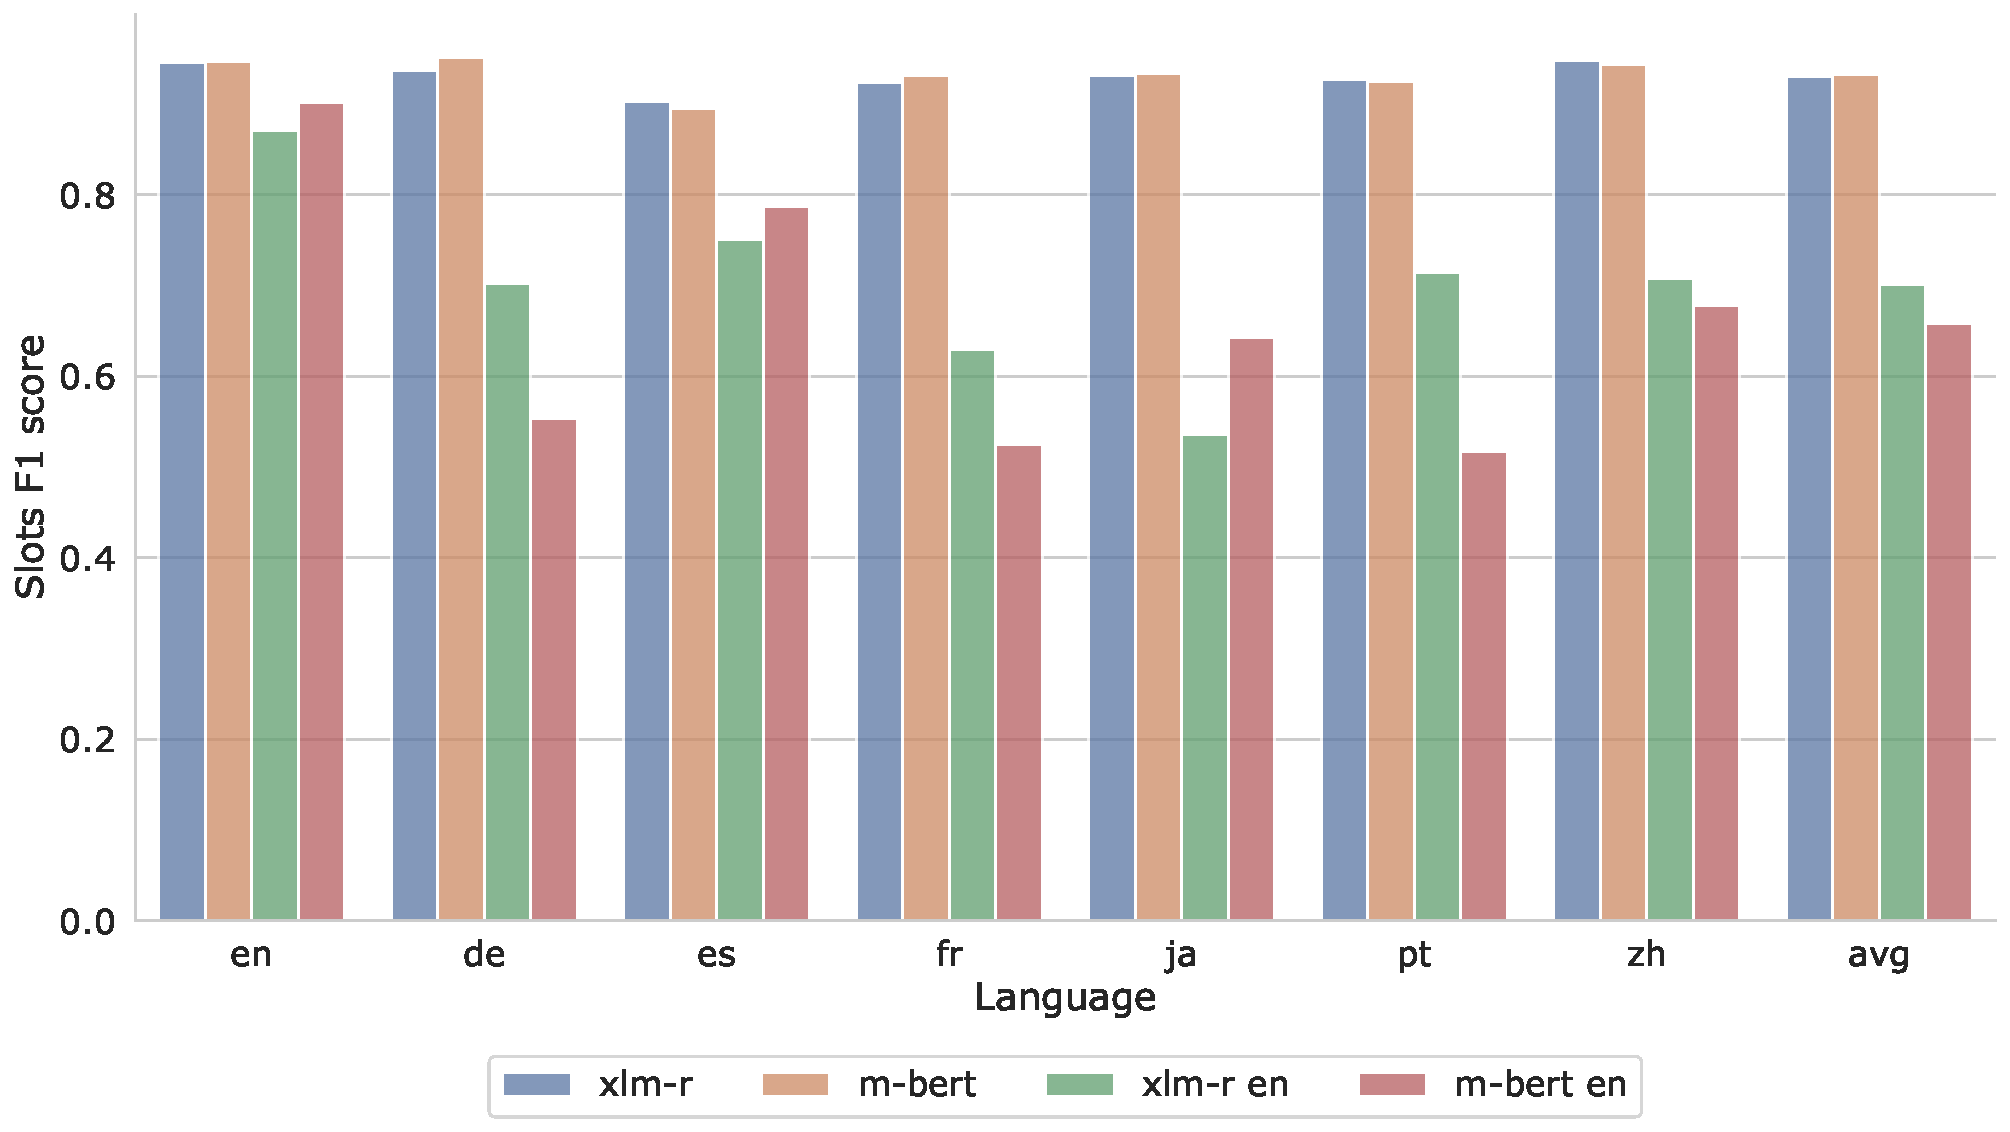
\includegraphics[width=\textwidth]{images/1}
    \caption{Сравнение моделей между собой \textbf{на тестовой выборке} датасета MultiAtis++ по метрике \textbf{Slots F1 score}.}\label{fig:figure1}
\end{figure}
\begin{figure}[H]
    \centering
    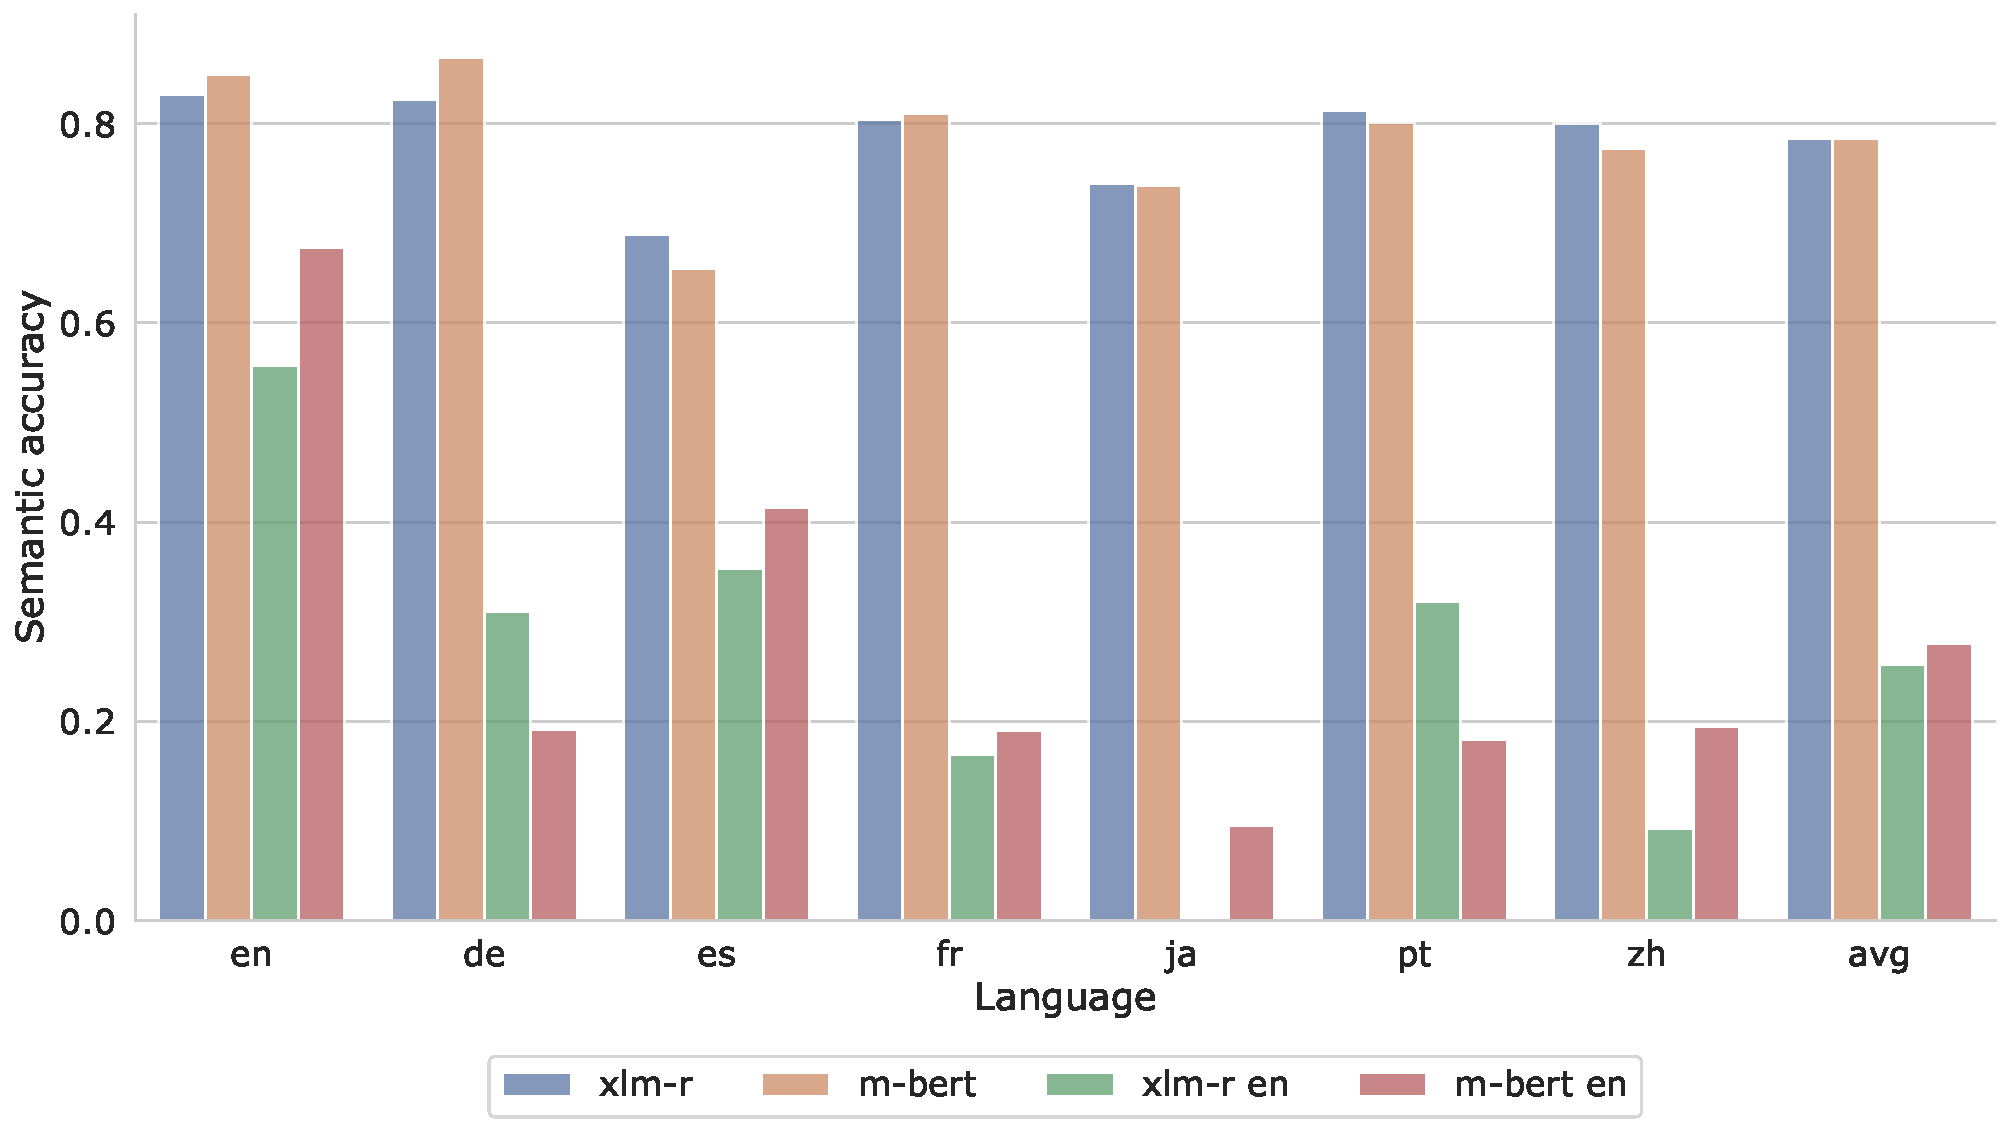
\includegraphics[width=\textwidth]{images/2}
    \caption{Сравнение моделей между собой \textbf{на тестовой выборке} датасета MultiAtis++ по метрике \textbf{Semantic accuracy}.}\label{fig:figure2}
\end{figure}

\begin{figure}[H]
    \centering
    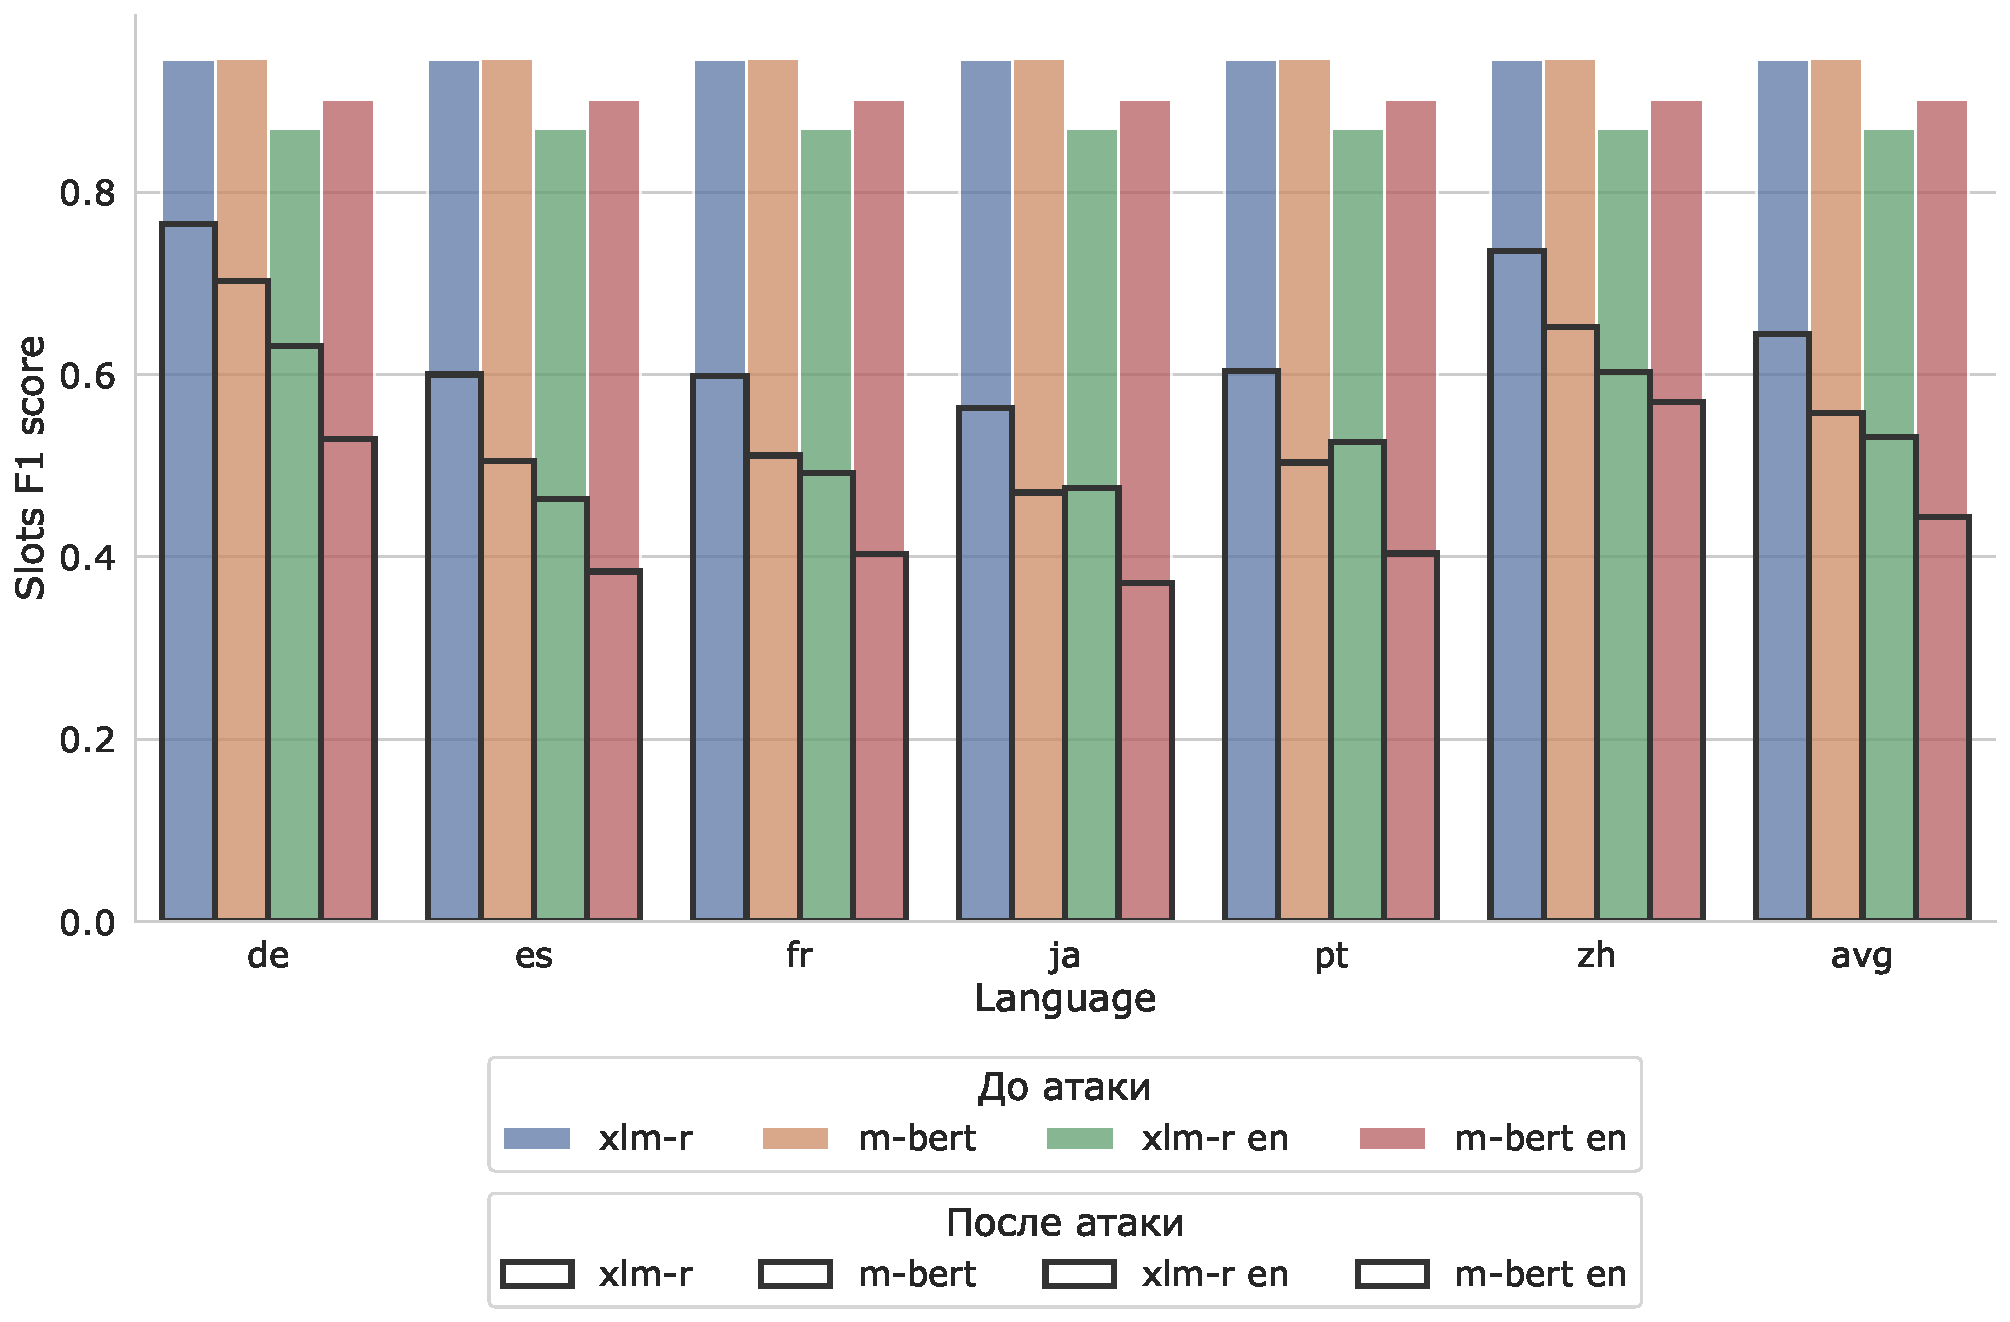
\includegraphics[width=\textwidth]{images/4}
    \caption{Сравнение моделей между собой после \textbf{word-level} атаки на тестовую выборку датасета MultiAtis++ по метрике \textbf{Slots F1 score}.}\label{fig:figure4}
\end{figure}
\begin{figure}[H]
    \centering
    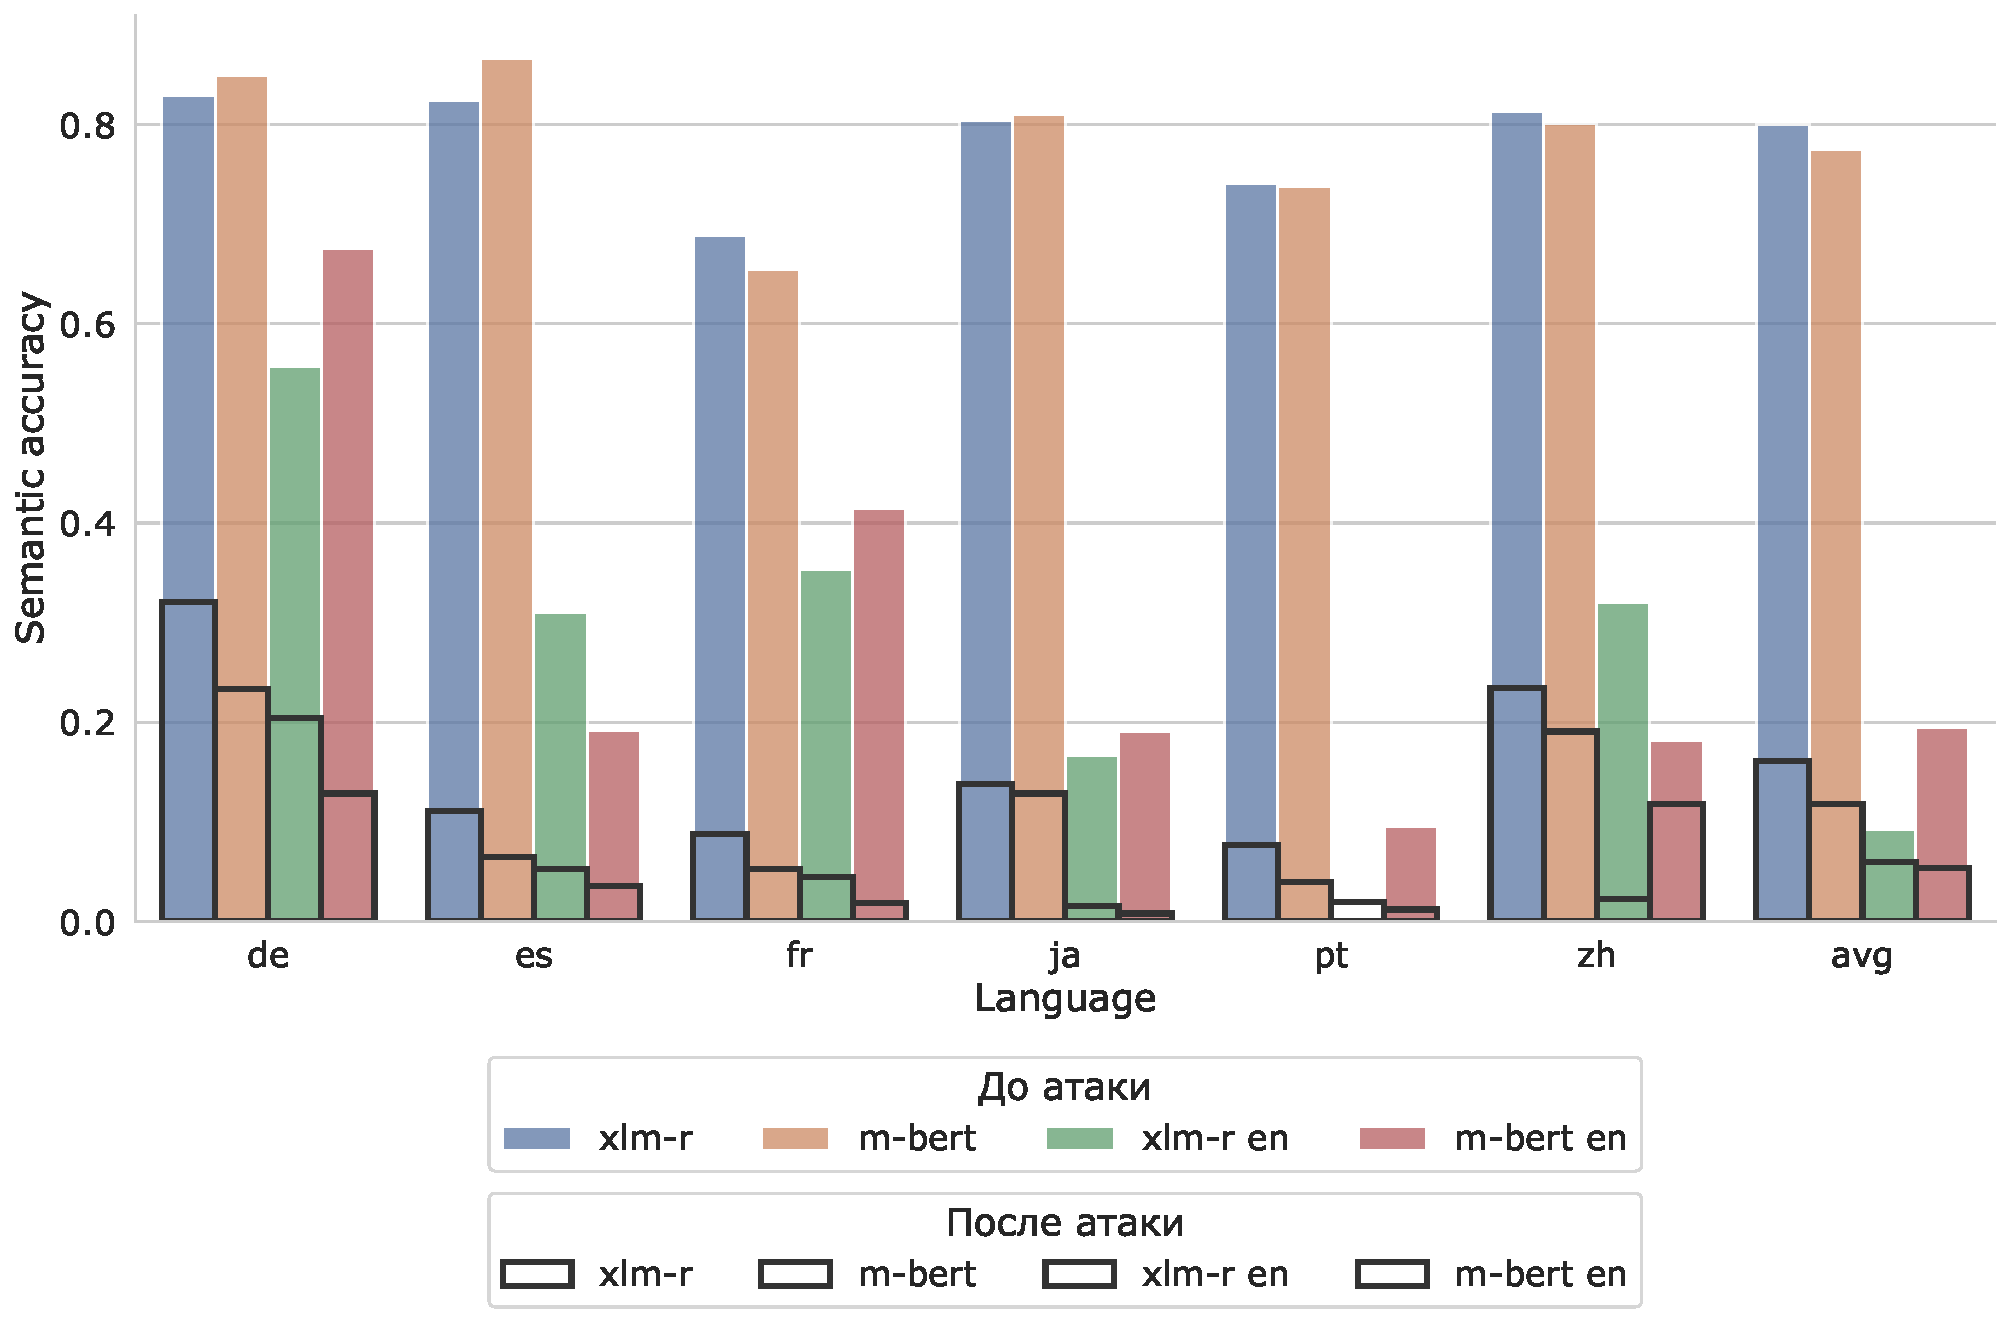
\includegraphics[width=\textwidth]{images/5}
    \caption{Сравнение моделей между собой после \textbf{word-level} атаки на тестовую выборку датасета MultiAtis++ по метрике \textbf{Semantic accuracy}.}\label{fig:figure5}
\end{figure}

\begin{figure}[H]
    \centering
    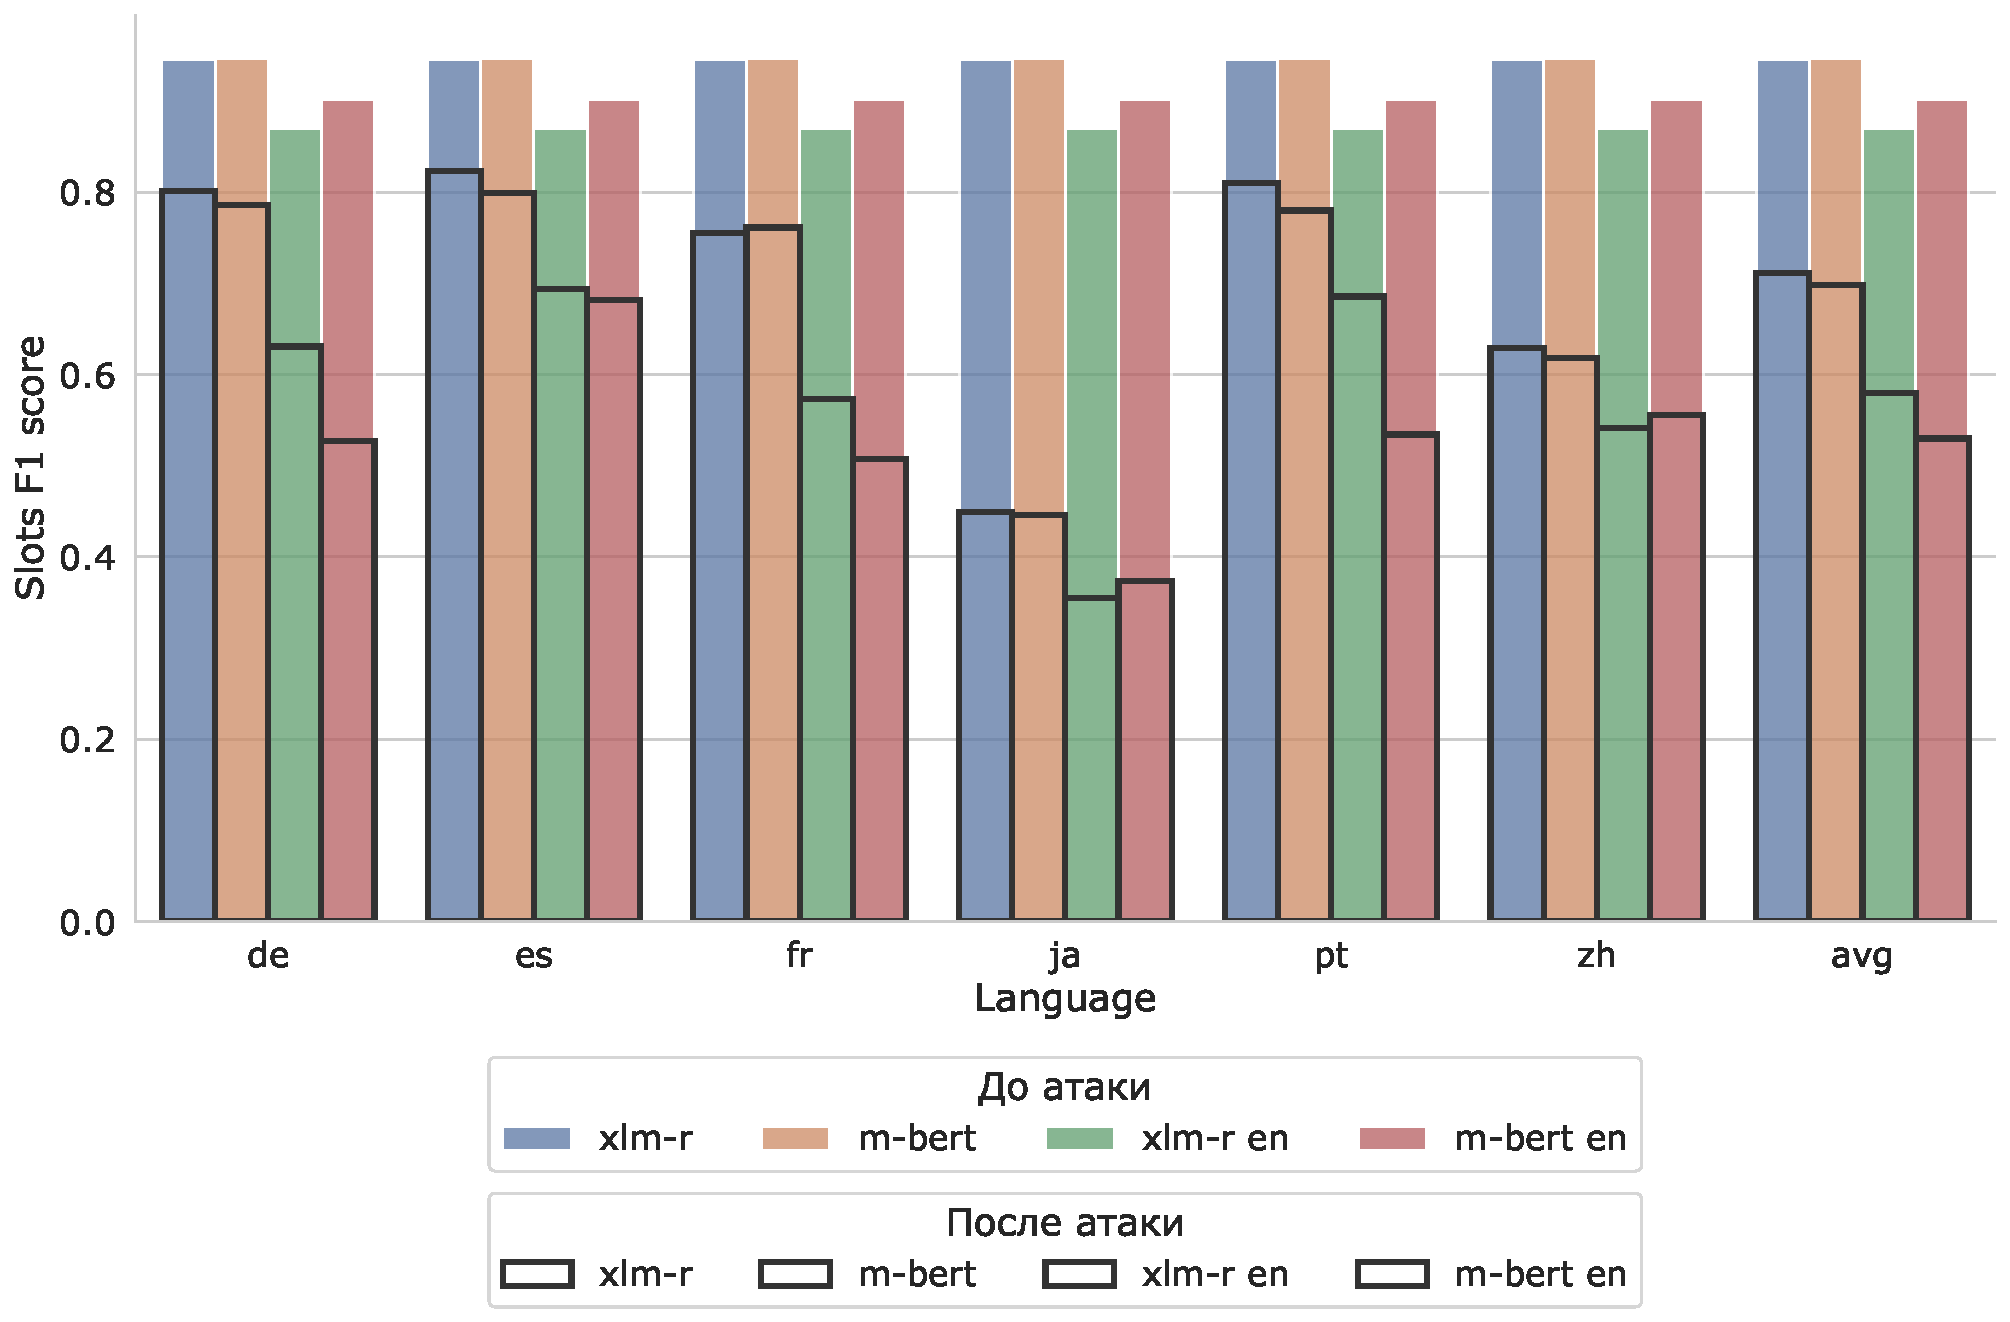
\includegraphics[width=\textwidth]{images/7}
    \caption{Сравнение моделей между собой после \textbf{phrase-level} атаки на тестовую выборку датасета MultiAtis++ по метрике \textbf{Slots F1 score}.}\label{fig:figure7}
\end{figure}
\begin{figure}[H]
    \centering
    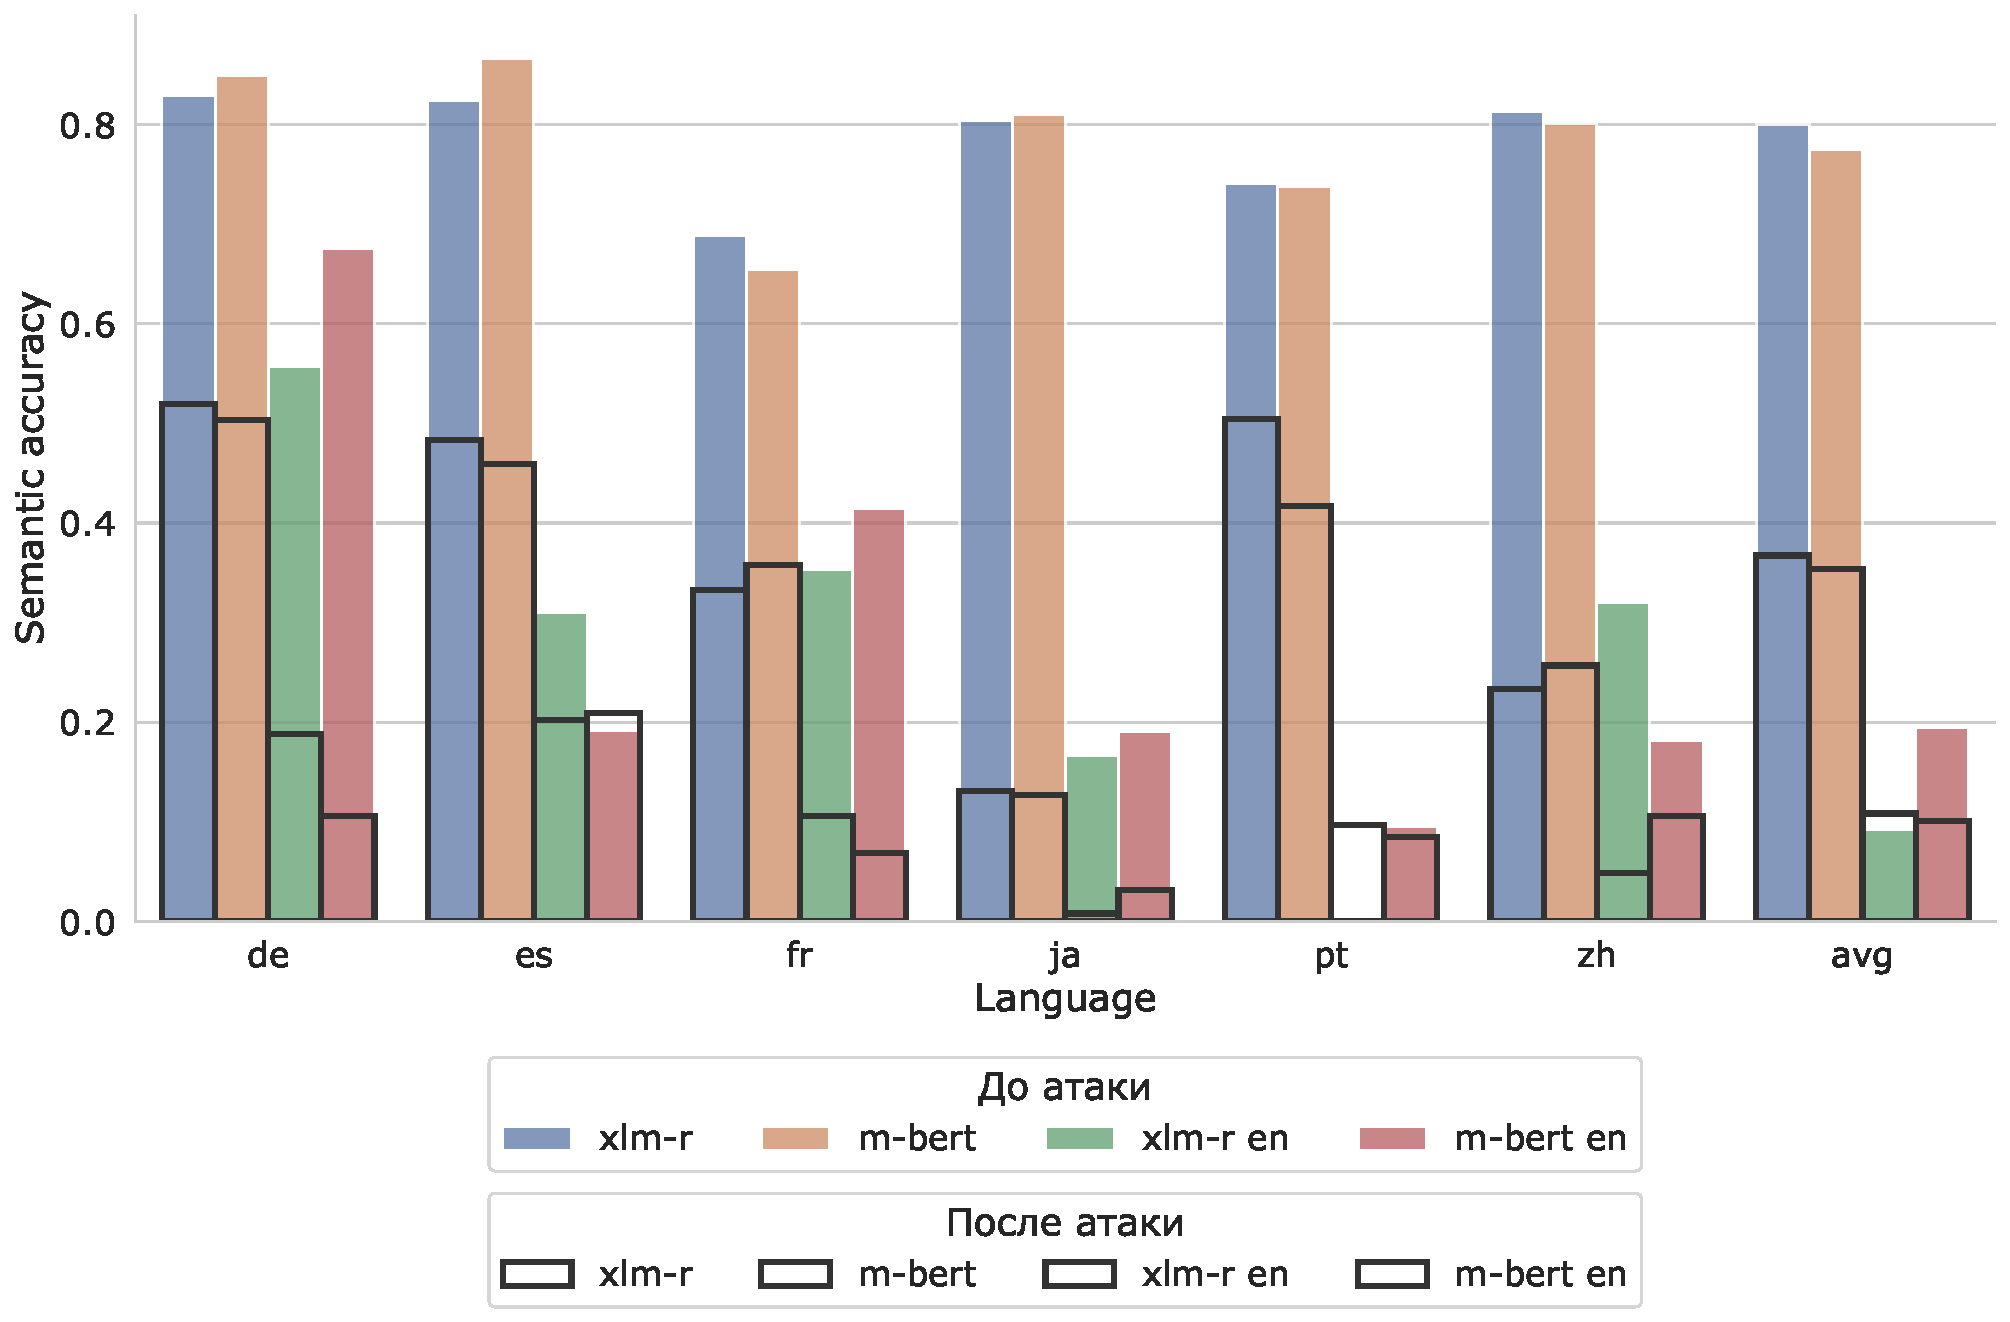
\includegraphics[width=\textwidth]{images/8}
    \caption{Сравнение моделей между собой после \textbf{phrase-level} атаки на тестовую выборку датасета MultiAtis++ по метрике \textbf{Semantic accuracy}.}\label{fig:figure8}
\end{figure}

\begin{figure}[H]
    \centering
    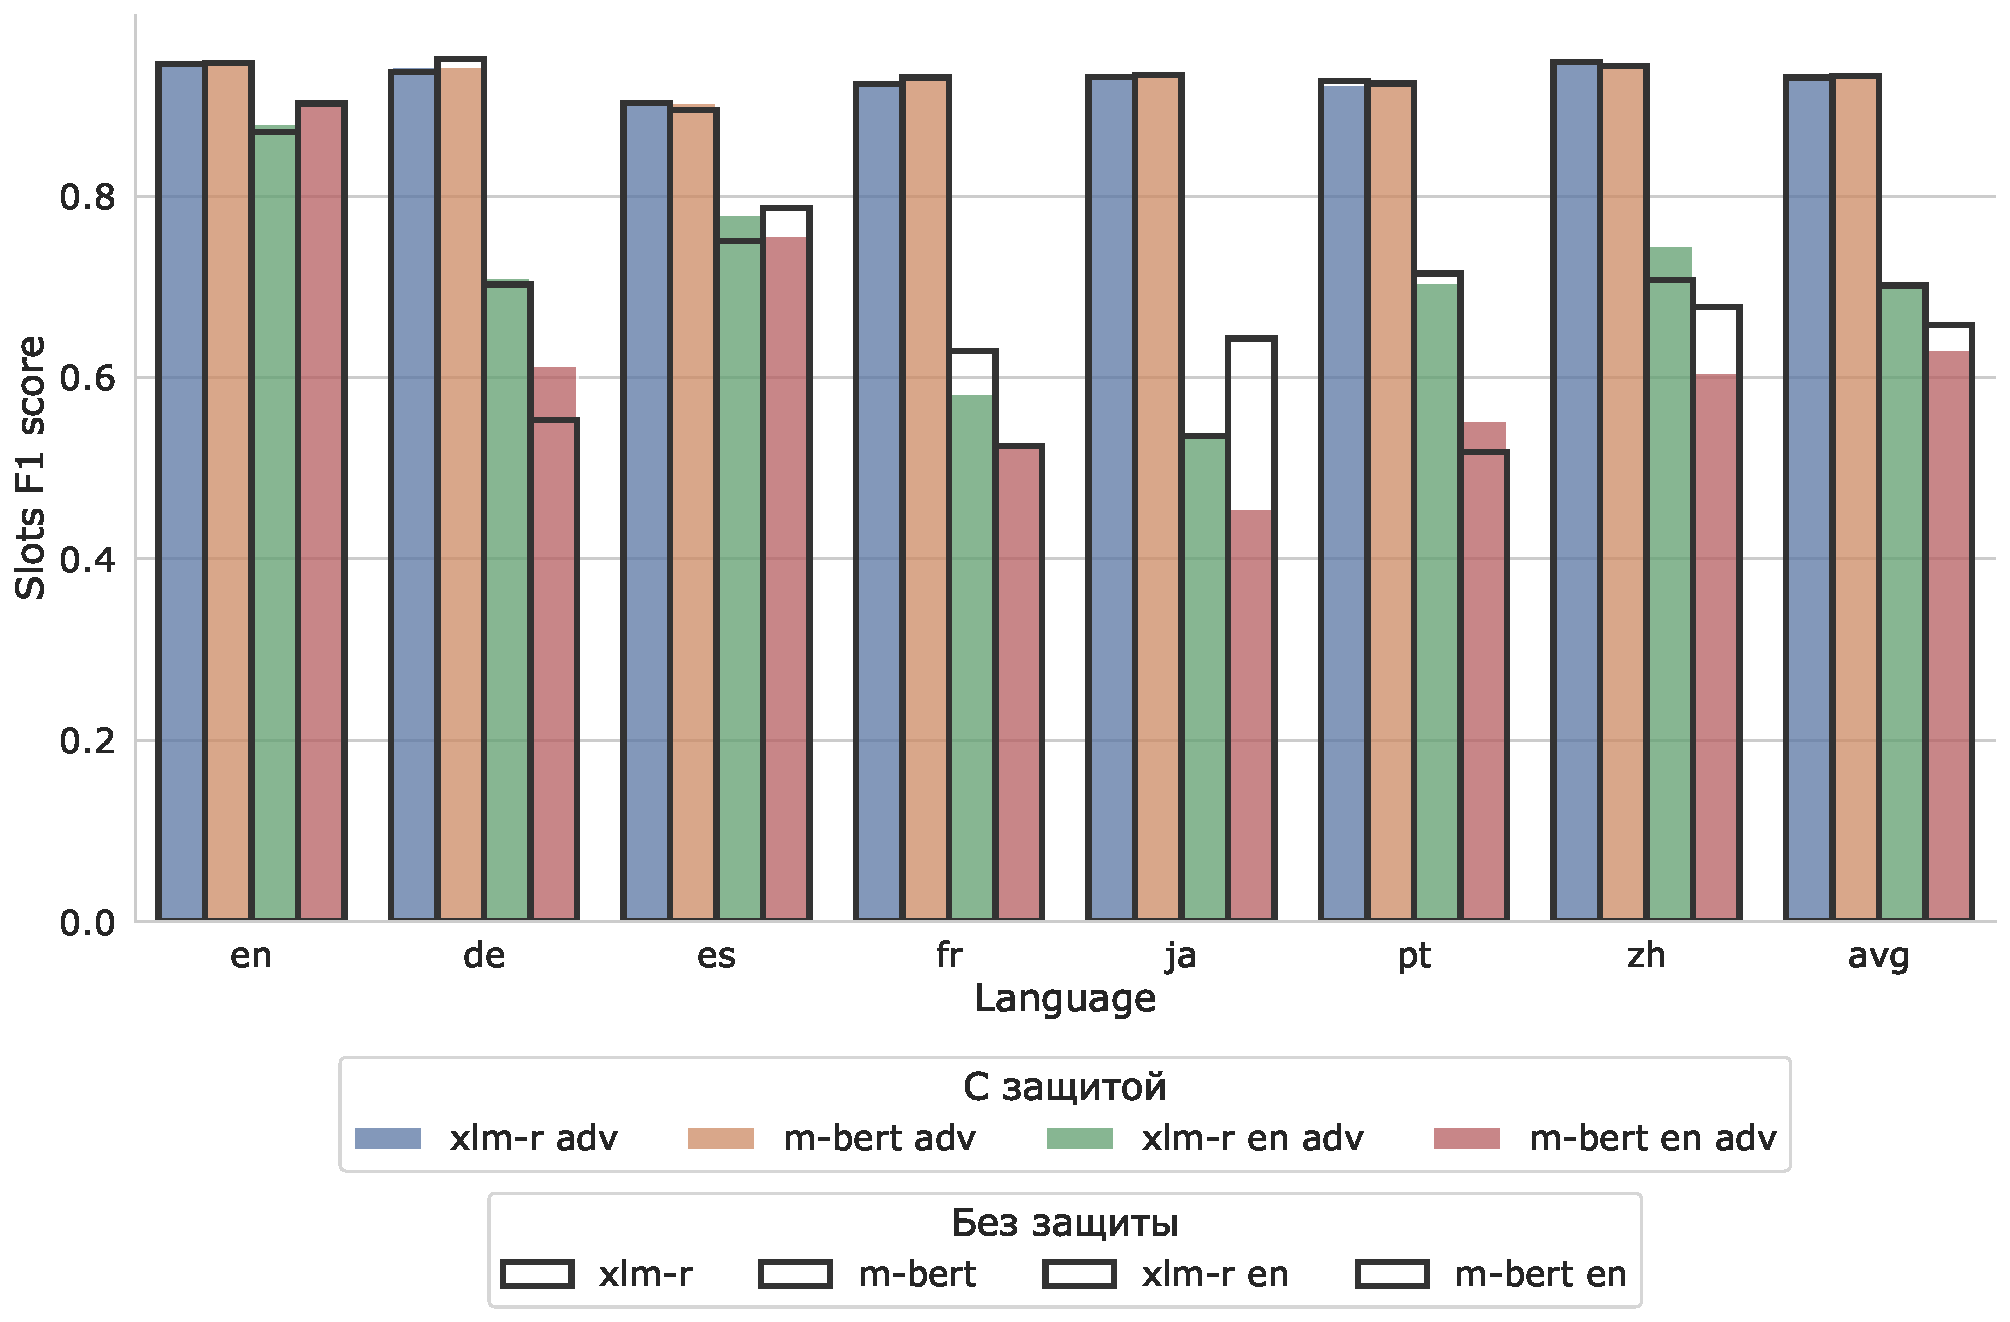
\includegraphics[width=\textwidth]{images/10}
    \caption{Сравнение моделей \textbf{с защитой} между собой \textbf{на тестовой выборке} датасета MultiAtis++ по метрике \textbf{Slots F1 score}.}\label{fig:figure10}
\end{figure}
\begin{figure}[H]
    \centering
    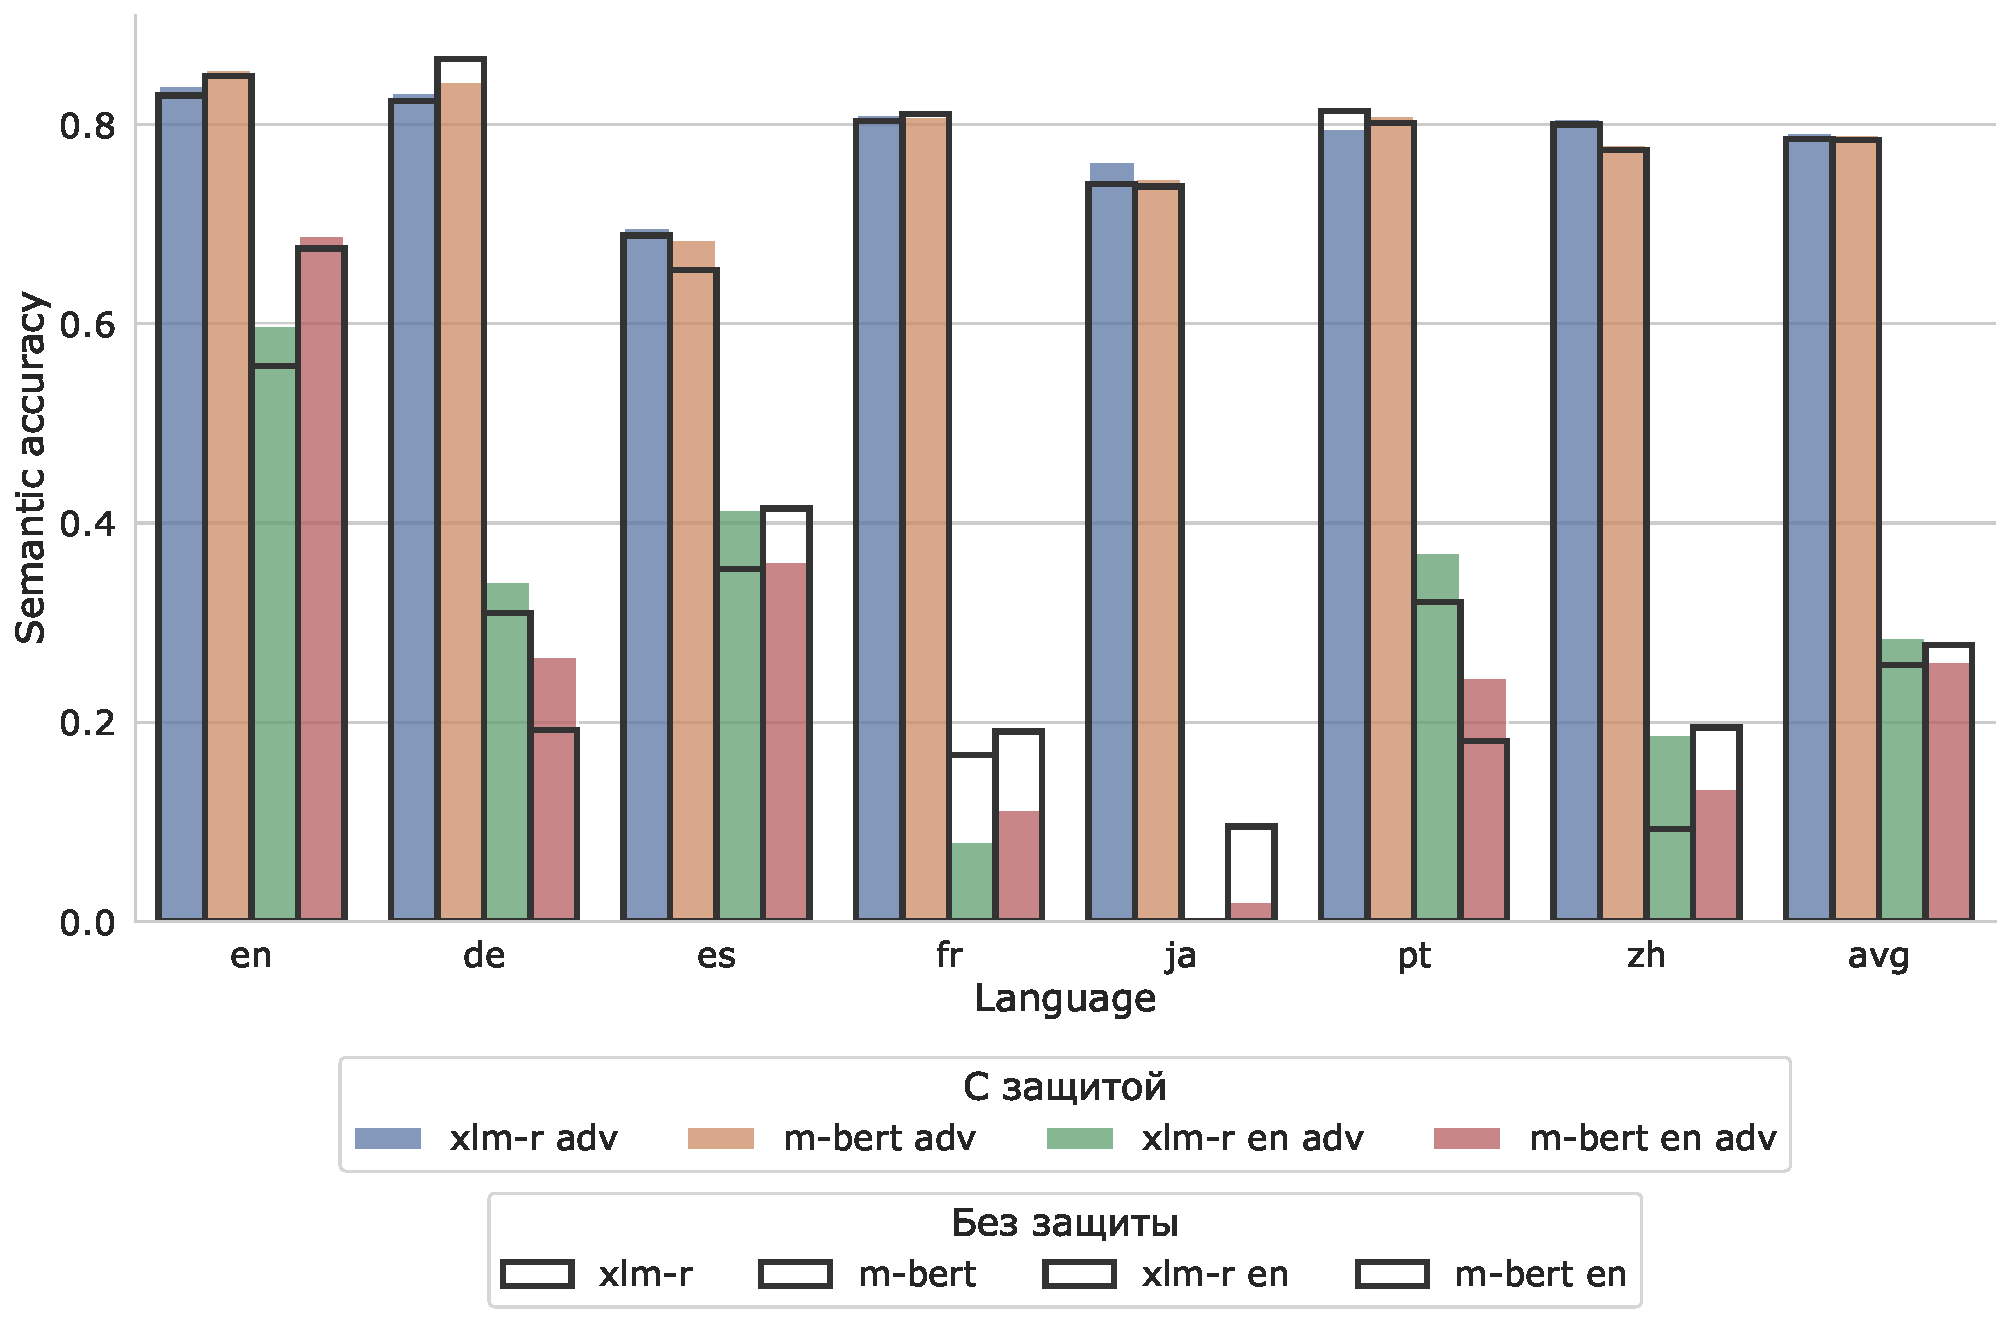
\includegraphics[width=\textwidth]{images/11}
    \caption{Сравнение моделей \textbf{с защитой} между собой \textbf{на тестовой выборке} датасета MultiAtis++ по метрике \textbf{Semantic accuracy}.}\label{fig:figure11}
\end{figure}

\begin{figure}[H]
    \centering
    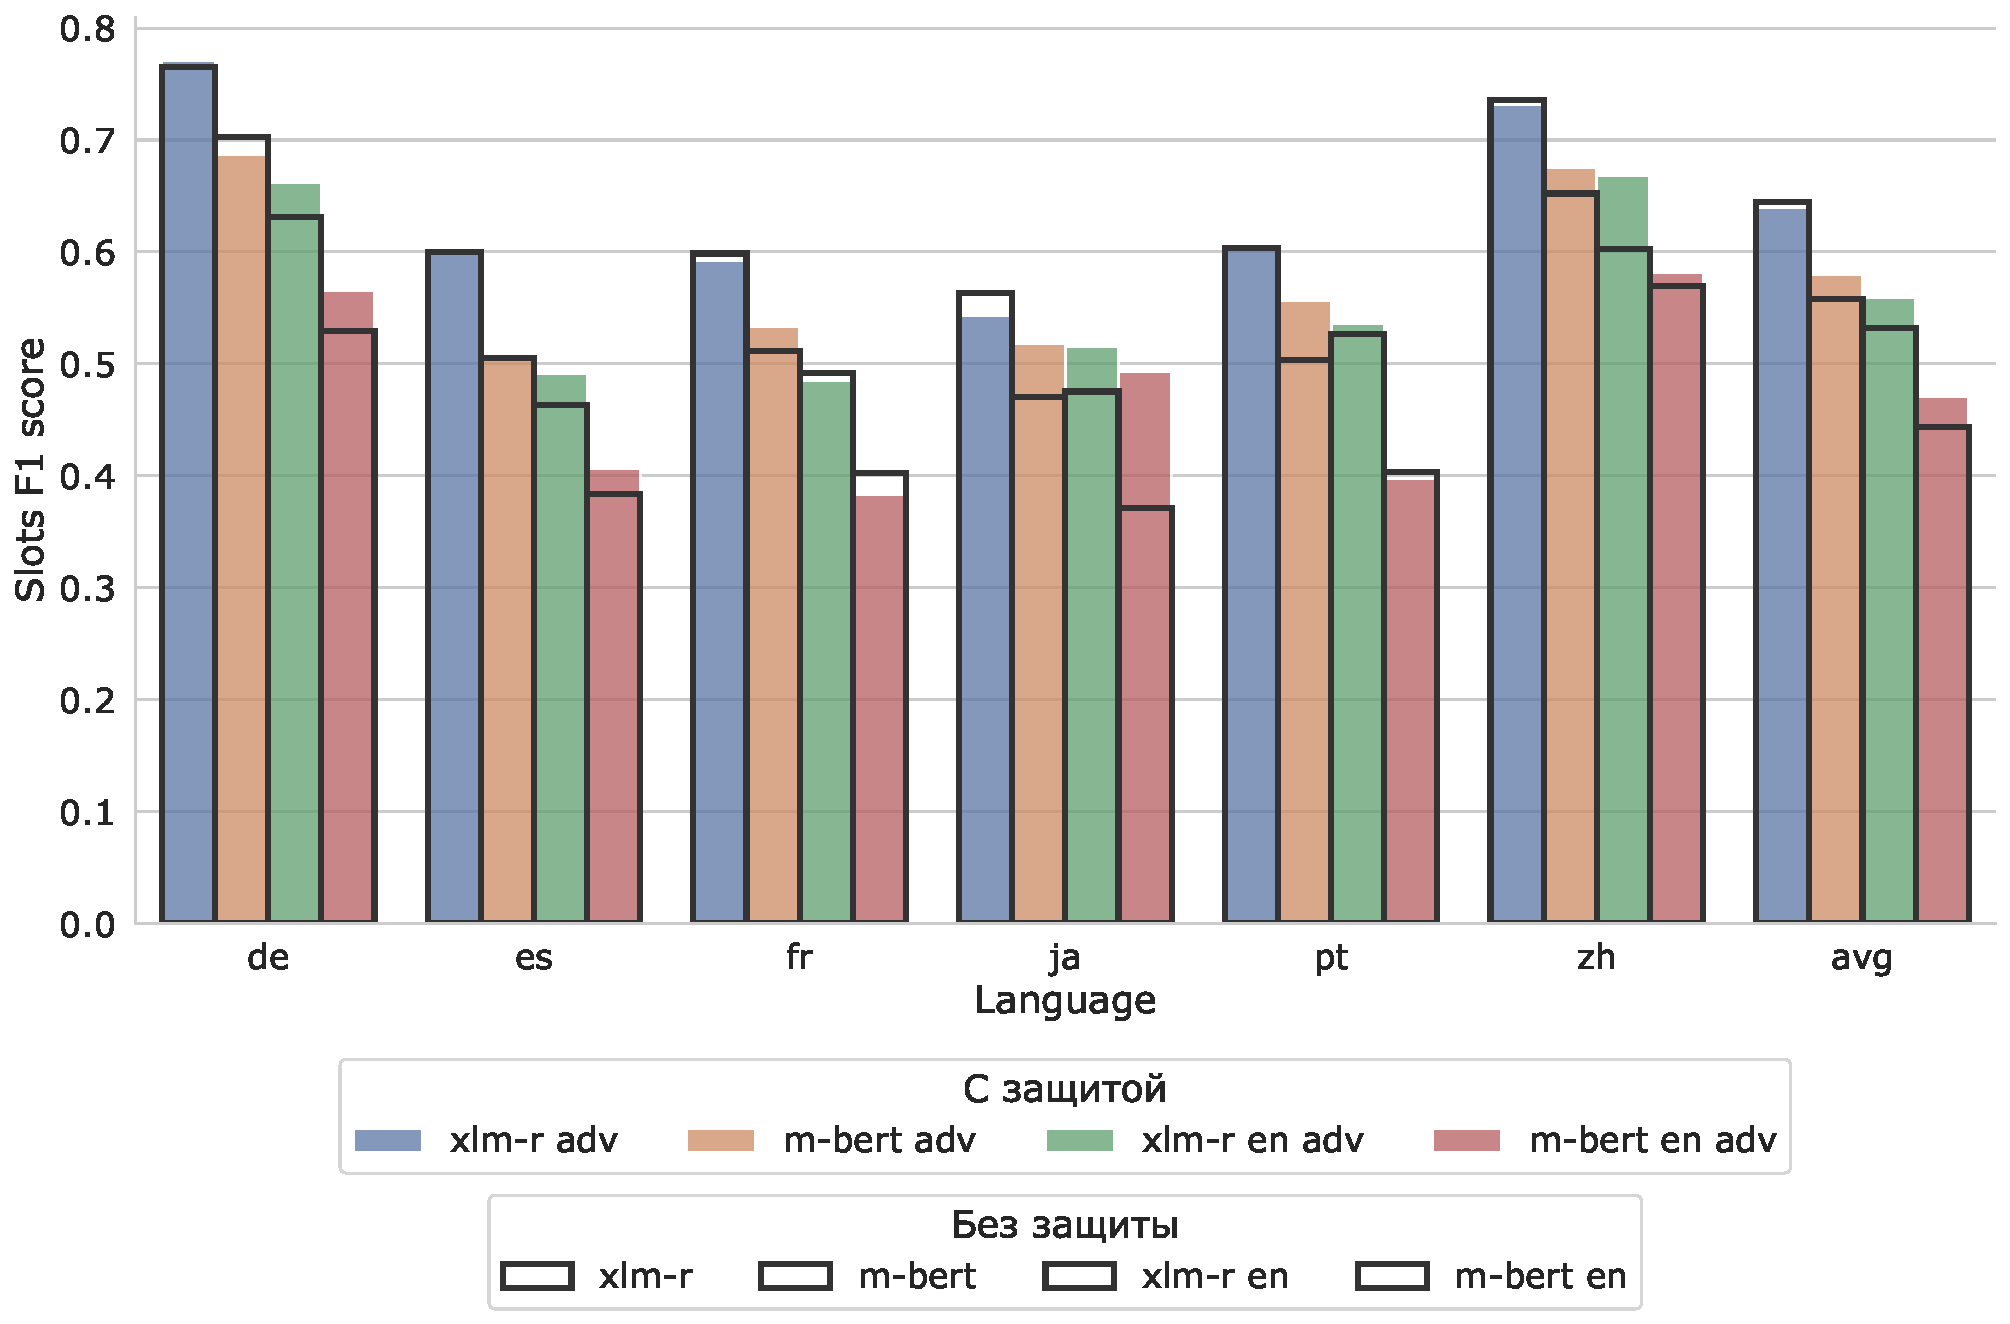
\includegraphics[width=\textwidth]{images/13}
    \caption{Сравнение моделей \textbf{с защитой} между собой после \textbf{word-level} атаки на тестовую выборку датасета MultiAtis++ по метрике \textbf{Slots F1 score}.}\label{fig:figure13}
\end{figure}
\begin{figure}[H]
    \centering
    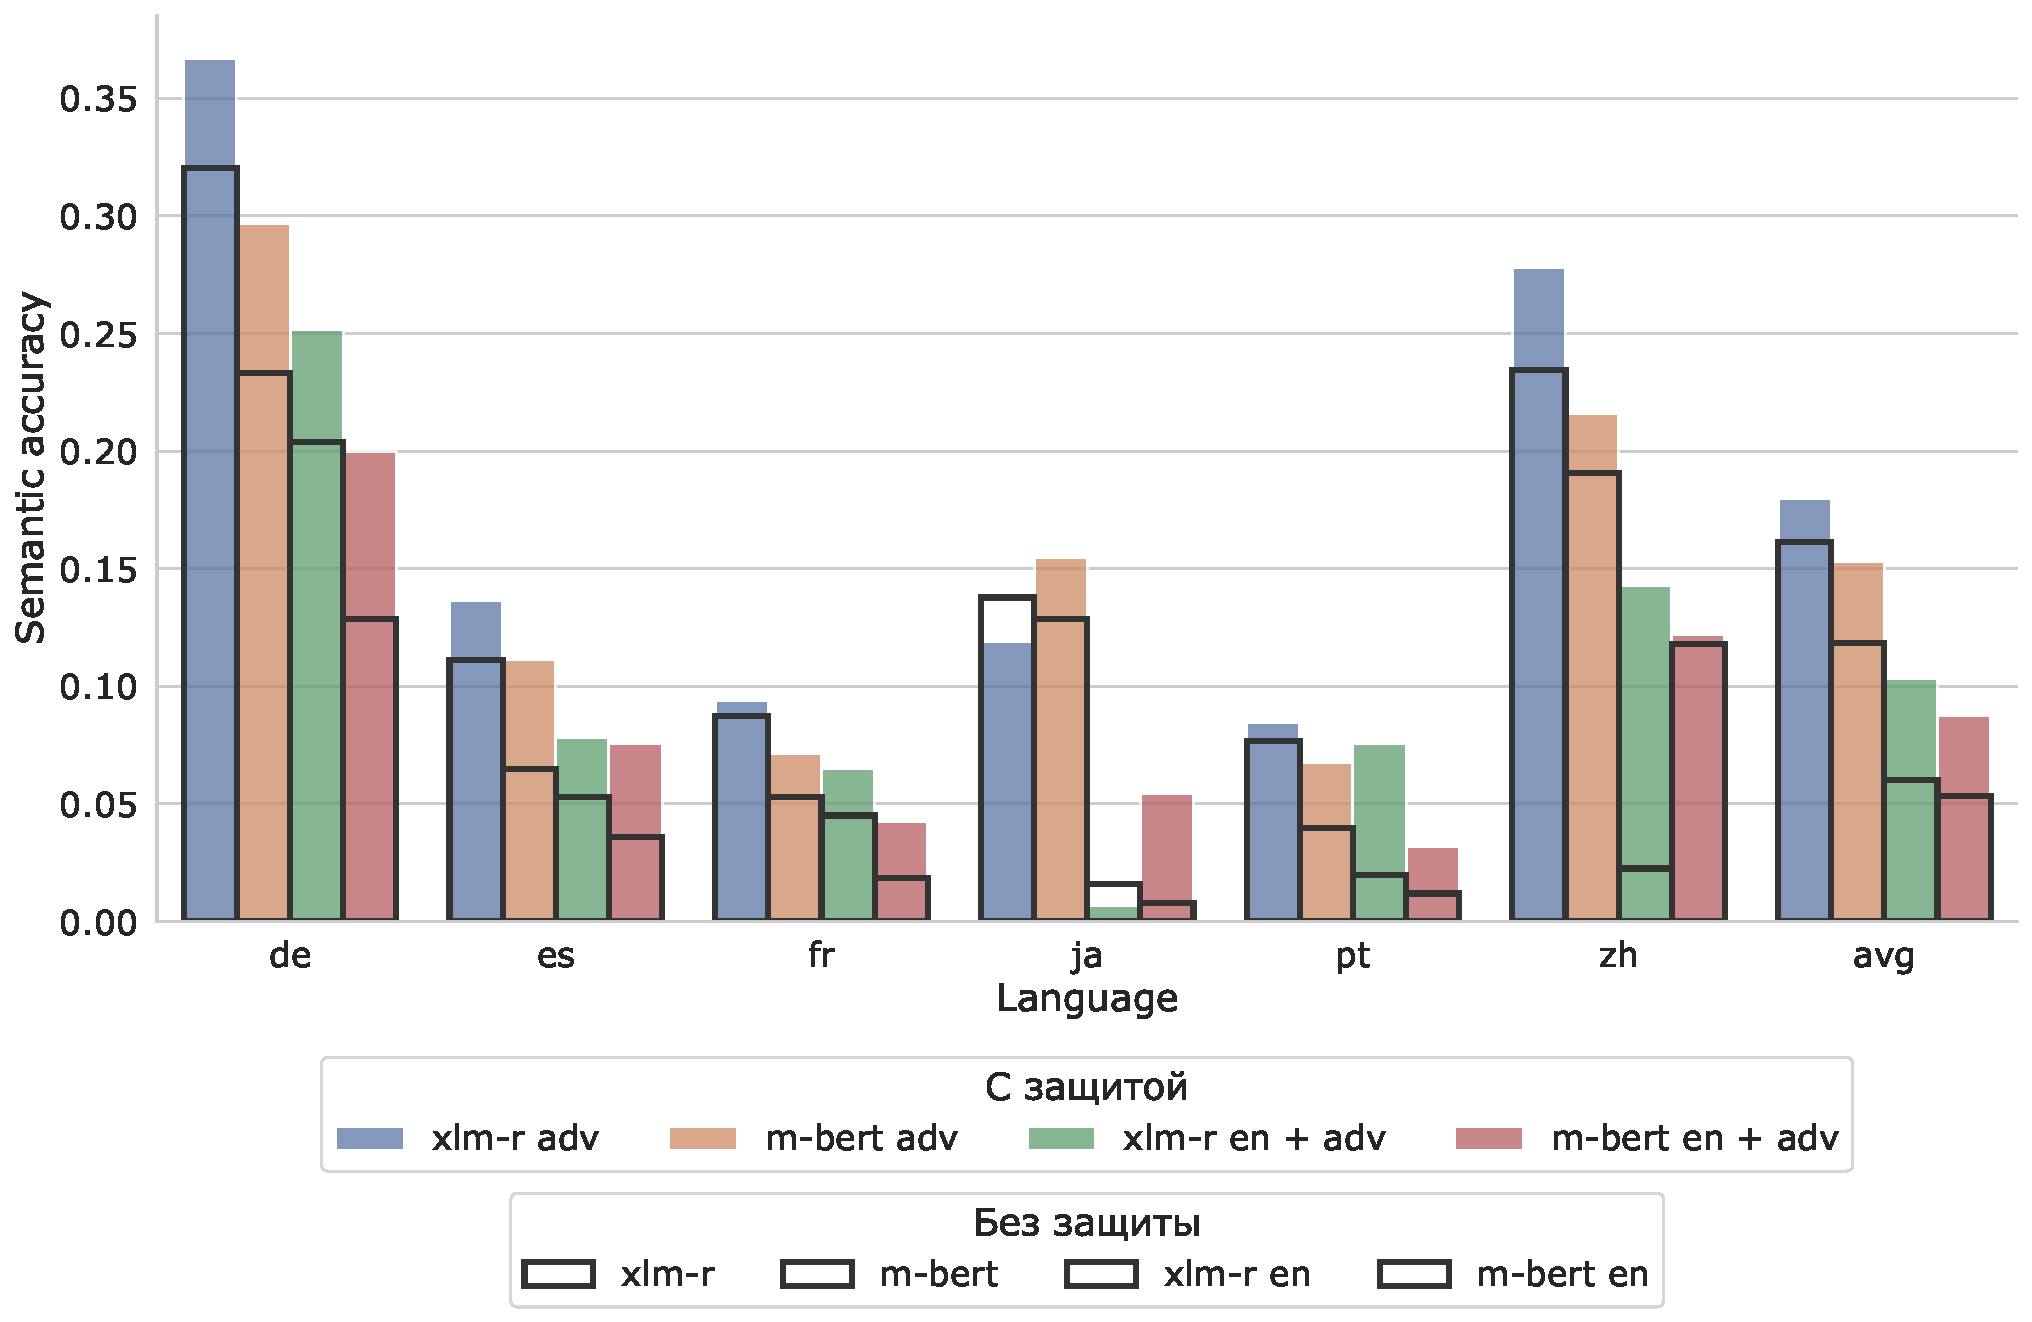
\includegraphics[width=\textwidth]{images/14}
    \caption{Сравнение моделей \textbf{с защитой} между собой после \textbf{word-level} атаки на тестовую выборку датасета MultiAtis++ по метрике \textbf{Semantic accuracy}.}\label{fig:figure14}
\end{figure}

\begin{figure}[H]
    \centering
    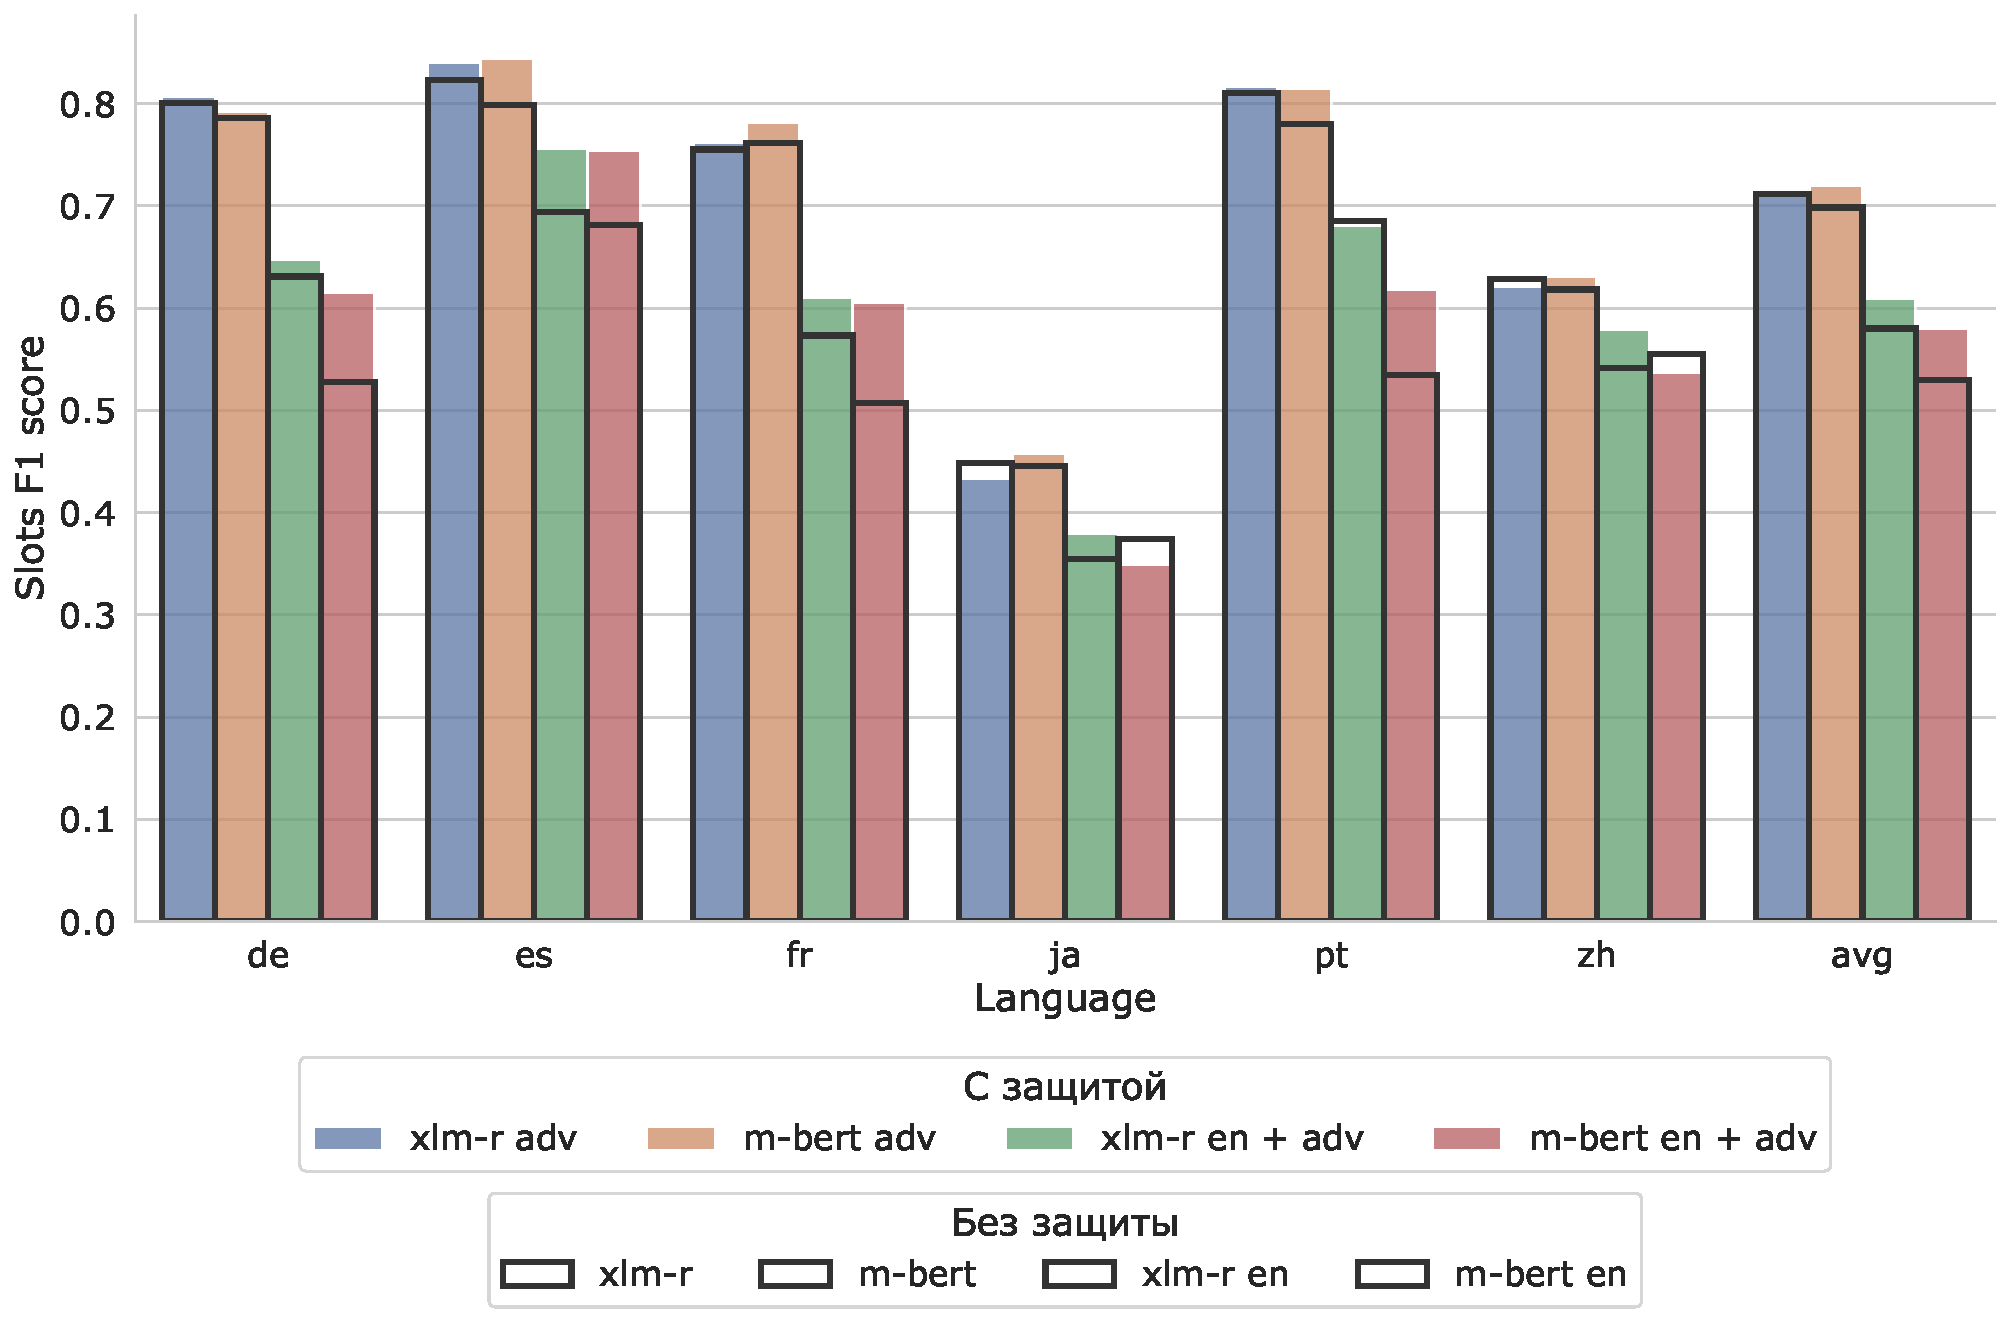
\includegraphics[width=\textwidth]{images/16}
    \caption{Сравнение моделей \textbf{с защитой} между собой после \textbf{phrase-level} атаки на тестовую выборку датасета MultiAtis++ по метрике \textbf{Slots F1 score}.}\label{fig:figure16}
\end{figure}
\begin{figure}[H]
    \centering
    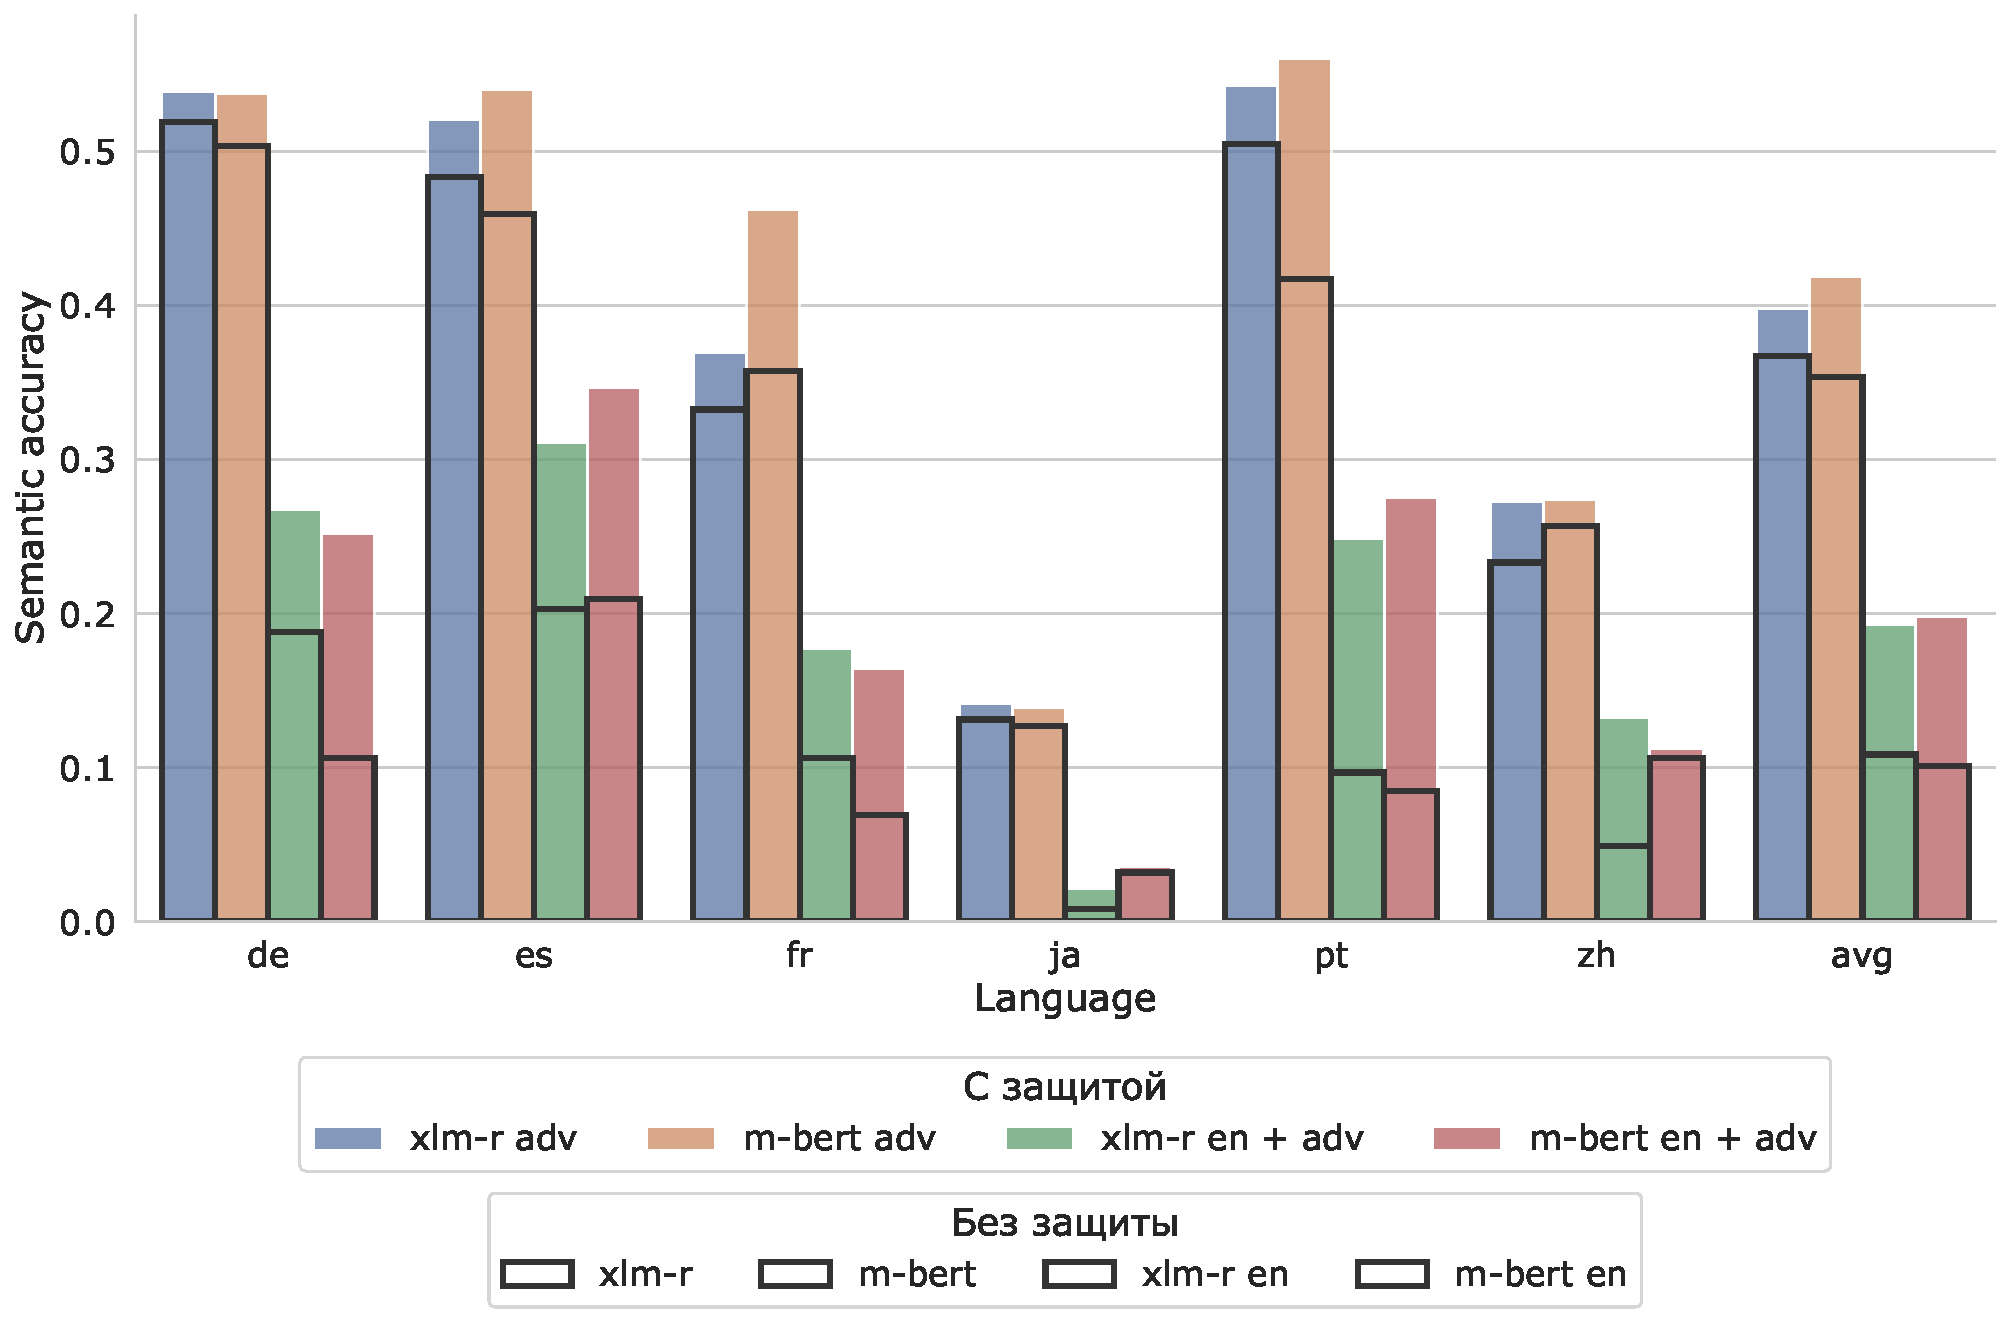
\includegraphics[width=\textwidth]{images/17}
    \caption{Сравнение моделей \textbf{с защитой} между собой после \textbf{phrase-level} атаки на тестовую выборку датасета MultiAtis++ по метрике \textbf{Semantic accuracy}.}\label{fig:figure17}
\end{figure}

\newpage

\subsection{Таблицы с результатами экспериментов}\label{subsec:tables}

\begin{table}[H]
	\resizebox{\textwidth}{!}{
		\begin{tabular}{|>{\bfseries}l|c|c|c|c|c|c|c|c|}
			\hline
			& en & de & es & fr & ja & pt & zh & avg \\ \hline
			xlm-r&$0.980$ & $0.975$ & $0.968$ & $0.972$ & $0.977$ & $0.970$ & $0.968$ & $0.973$ \\ \hline
			m-bert&$0.977$ & $0.977$ & $0.963$ & $0.966$ & $0.959$ & $0.967$ & $0.962$ & $0.967$ \\ \hline
			xlm-r en&$0.903$ & $0.885$ & $0.882$ & $0.879$ & $0.830$ & $0.846$ & $0.856$ & $0.869$ \\ \hline
			m-bert en&$0.951$ & $0.828$ & $0.865$ & $0.877$ & $0.750$ & $0.853$ & $0.795$ & $0.845$ \\ \hline
		\end{tabular}
	}\caption{Сравнение моделей между собой \textbf{на тестовой выборке} датасета MultiAtis++ по метрике \textbf{Intent accuracy}. По колонкам языки тестовых подвыборок, по рядам тестируемые модели.}\label{tab:table0}
\end{table}
\begin{table}[H]
	\resizebox{\textwidth}{!}{
		\begin{tabular}{|>{\bfseries}l|c|c|c|c|c|c|c|c|}
			\hline
			& en & de & es & fr & ja & pt & zh & avg \\ \hline
			xlm-r&$0.945$ & $0.937$ & $0.902$ & $0.924$ & $0.931$ & $0.927$ & $0.948$ & $0.931$ \\ \hline
			m-bert&$0.947$ & $0.951$ & $0.895$ & $0.931$ & $0.933$ & $0.924$ & $0.944$ & $0.932$ \\ \hline
			xlm-r en&$0.871$ & $0.702$ & $0.750$ & $0.629$ & $0.535$ & $0.715$ & $0.707$ & $0.701$ \\ \hline
			m-bert en&$0.902$ & $0.553$ & $0.787$ & $0.524$ & $0.643$ & $0.517$ & $0.678$ & $0.658$ \\ \hline
		\end{tabular}
	}\caption{Сравнение моделей между собой \textbf{на тестовой выборке} датасета MultiAtis++ по метрике \textbf{Slots F1 score}. По колонкам языки тестовых подвыборок, по рядам тестируемые модели.}\label{tab:table1}
\end{table}
\begin{table}[H]
	\resizebox{\textwidth}{!}{
		\begin{tabular}{|>{\bfseries}l|c|c|c|c|c|c|c|c|}
			\hline
			& en & de & es & fr & ja & pt & zh & avg \\ \hline
			xlm-r&$0.829$ & $0.824$ & $0.689$ & $0.804$ & $0.740$ & $0.813$ & $0.800$ & $0.786$ \\ \hline
			m-bert&$0.849$ & $0.866$ & $0.654$ & $0.811$ & $0.738$ & $0.801$ & $0.775$ & $0.785$ \\ \hline
			xlm-r en&$0.558$ & $0.310$ & $0.354$ & $0.167$ & $0.000$ & $0.321$ & $0.093$ & $0.257$ \\ \hline
			m-bert en&$0.675$ & $0.192$ & $0.415$ & $0.191$ & $0.095$ & $0.181$ & $0.195$ & $0.278$ \\ \hline
		\end{tabular}
	}\caption{Сравнение моделей между собой \textbf{на тестовой выборке} датасета MultiAtis++ по метрике \textbf{Semantic accuracy}. По колонкам языки тестовых подвыборок, по рядам тестируемые модели.}\label{tab:table2}
\end{table}

\begin{table}[H]
	\resizebox{\textwidth}{!}{
		\begin{tabular}{|>{\bfseries}l|c|c|c|c|c|c|c|}
			\hline
			& de & es & fr & ja & pt & zh & avg \\ \hline
			xlm-r&$0.931$ & $0.877$ & $0.849$ & $0.825$ & $0.901$ & $0.872$ & $0.876$ \\ \hline
			m-bert&$0.893$ & $0.891$ & $0.872$ & $0.820$ & $0.853$ & $0.852$ & $0.863$ \\ \hline
			xlm-r en&$0.809$ & $0.783$ & $0.774$ & $0.677$ & $0.554$ & $0.728$ & $0.721$ \\ \hline
			m-bert en&$0.811$ & $0.760$ & $0.793$ & $0.723$ & $0.760$ & $0.777$ & $0.771$ \\ \hline
		\end{tabular}
	}\caption{Сравнение моделей между собой после word-level атаки на тестовую выборку датасета MultiAtis++ по метрике \textbf{Intent accuracy}. По колонкам встраиваемые языки, по рядам тестируемые модели.}\label{tab:table3}
\end{table}
\begin{table}[H]
	\resizebox{\textwidth}{!}{
		\begin{tabular}{|>{\bfseries}l|c|c|c|c|c|c|c|}
			\hline
			& de & es & fr & ja & pt & zh & avg \\ \hline
			xlm-r&$0.767$ & $0.589$ & $0.603$ & $0.552$ & $0.598$ & $0.747$ & $0.642$ \\ \hline
			m-bert&$0.685$ & $0.517$ & $0.510$ & $0.428$ & $0.494$ & $0.684$ & $0.553$ \\ \hline
			xlm-r en&$0.642$ & $0.467$ & $0.499$ & $0.508$ & $0.543$ & $0.641$ & $0.550$ \\ \hline
			m-bert en&$0.539$ & $0.385$ & $0.419$ & $0.362$ & $0.391$ & $0.585$ & $0.447$ \\ \hline
		\end{tabular}
	}\caption{Сравнение моделей между собой после word-level атаки на тестовую выборку датасета MultiAtis++ по метрике \textbf{Slots F1 score}. По колонкам встраиваемые языки, по рядам тестируемые модели.}\label{tab:table4}
\end{table}
\begin{table}[H]
	\resizebox{\textwidth}{!}{
		\begin{tabular}{|>{\bfseries}l|c|c|c|c|c|c|c|}
			\hline
			& de & es & fr & ja & pt & zh & avg \\ \hline
			xlm-r&$0.343$ & $0.109$ & $0.086$ & $0.170$ & $0.077$ & $0.278$ & $0.177$ \\ \hline
			m-bert&$0.228$ & $0.083$ & $0.058$ & $0.081$ & $0.038$ & $0.213$ & $0.117$ \\ \hline
			xlm-r en&$0.201$ & $0.057$ & $0.056$ & $0.013$ & $0.023$ & $0.042$ & $0.065$ \\ \hline
			m-bert en&$0.136$ & $0.029$ & $0.032$ & $0.005$ & $0.011$ & $0.115$ & $0.055$ \\ \hline
		\end{tabular}
	}\caption{Сравнение моделей между собой после word-level атаки на тестовую выборку датасета MultiAtis++ по метрике \textbf{Semantic accuracy}. По колонкам встраиваемые языки, по рядам тестируемые модели.}\label{tab:table5}
\end{table}

\begin{table}[H]
	\resizebox{\textwidth}{!}{
		\begin{tabular}{|>{\bfseries}l|c|c|c|c|c|c|c|}
			\hline
			& de & es & fr & ja & pt & zh & avg \\ \hline
			xlm-r&$0.954$ & $0.946$ & $0.928$ & $0.952$ & $0.964$ & $0.950$ & $0.949$ \\ \hline
			m-bert&$0.948$ & $0.935$ & $0.939$ & $0.951$ & $0.940$ & $0.934$ & $0.941$ \\ \hline
			xlm-r en&$0.808$ & $0.836$ & $0.740$ & $0.750$ & $0.442$ & $0.784$ & $0.727$ \\ \hline
			m-bert en&$0.809$ & $0.833$ & $0.834$ & $0.805$ & $0.861$ & $0.829$ & $0.829$ \\ \hline
		\end{tabular}
	}\caption{Сравнение моделей между собой после phrase-level атаки на тестовую выборку датасета MultiAtis++ по метрике \textbf{Intent accuracy}. По колонкам встраиваемые языки, по рядам тестируемые модели.}\label{tab:table6}
\end{table}
\begin{table}[H]
	\resizebox{\textwidth}{!}{
		\begin{tabular}{|>{\bfseries}l|c|c|c|c|c|c|c|}
			\hline
			& de & es & fr & ja & pt & zh & avg \\ \hline
			xlm-r&$0.802$ & $0.829$ & $0.751$ & $0.444$ & $0.813$ & $0.609$ & $0.708$ \\ \hline
			m-bert&$0.784$ & $0.804$ & $0.758$ & $0.450$ & $0.783$ & $0.619$ & $0.700$ \\ \hline
			xlm-r en&$0.627$ & $0.704$ & $0.569$ & $0.365$ & $0.680$ & $0.561$ & $0.584$ \\ \hline
			m-bert en&$0.539$ & $0.699$ & $0.531$ & $0.366$ & $0.530$ & $0.563$ & $0.538$ \\ \hline
		\end{tabular}
	}\caption{Сравнение моделей между собой после phrase-level атаки на тестовую выборку датасета MultiAtis++ по метрике \textbf{Slots F1 score}. По колонкам встраиваемые языки, по рядам тестируемые модели.}\label{tab:table7}
\end{table}
\begin{table}[H]
	\resizebox{\textwidth}{!}{
		\begin{tabular}{|>{\bfseries}l|c|c|c|c|c|c|c|}
			\hline
			& de & es & fr & ja & pt & zh & avg \\ \hline
			xlm-r&$0.511$ & $0.511$ & $0.336$ & $0.115$ & $0.522$ & $0.209$ & $0.368$ \\ \hline
			m-bert&$0.487$ & $0.438$ & $0.344$ & $0.114$ & $0.433$ & $0.256$ & $0.345$ \\ \hline
			xlm-r en&$0.163$ & $0.229$ & $0.099$ & $0.013$ & $0.070$ & $0.064$ & $0.106$ \\ \hline
			m-bert en&$0.122$ & $0.219$ & $0.085$ & $0.041$ & $0.087$ & $0.106$ & $0.110$ \\ \hline
		\end{tabular}
	}\caption{Сравнение моделей между собой после phrase-level атаки на тестовую выборку датасета MultiAtis++ по метрике \textbf{Semantic accuracy}. По колонкам встраиваемые языки, по рядам тестируемые модели.}\label{tab:table8}
\end{table}

\begin{table}[H]
	\resizebox{\textwidth}{!}{
		\begin{tabular}{|>{\bfseries}l|c|c|c|c|c|c|c|c|}
			\hline
			& en & de & es & fr & ja & pt & zh & avg \\ \hline
			xlm-r adv&$0.981$ & $0.974$ & $0.964$ & $0.976$ & $0.972$ & $0.967$ & $0.967$ & $0.972$ \\ \hline
			m-bert adv&$0.975$ & $0.976$ & $0.964$ & $0.972$ & $0.960$ & $0.970$ & $0.962$ & $0.968$ \\ \hline
			xlm-r en + adv&$0.928$ & $0.890$ & $0.913$ & $0.872$ & $0.789$ & $0.881$ & $0.816$ & $0.870$ \\ \hline
			m-bert en + adv&$0.959$ & $0.848$ & $0.901$ & $0.893$ & $0.719$ & $0.901$ & $0.759$ & $0.854$ \\ \hline
		\end{tabular}
	}\caption{Сравнение моделей с защитой между собой на тестовой выборке датасета MultiAtis++ по метрике \textbf{Intent accuracy}. По колонкам языки тестовых подвыборок, по рядам тестируемые модели.}\label{tab:table9}
\end{table}
\begin{table}[H]
	\resizebox{\textwidth}{!}{
		\begin{tabular}{|>{\bfseries}l|c|c|c|c|c|c|c|c|}
			\hline
			& en & de & es & fr & ja & pt & zh & avg \\ \hline
			xlm-r adv&$0.947$ & $0.940$ & $0.906$ & $0.929$ & $0.928$ & $0.929$ & $0.946$ & $0.932$ \\ \hline
			m-bert adv&$0.950$ & $0.942$ & $0.900$ & $0.928$ & $0.935$ & $0.920$ & $0.946$ & $0.932$ \\ \hline
			xlm-r en + adv&$0.888$ & $0.729$ & $0.788$ & $0.623$ & $0.447$ & $0.743$ & $0.718$ & $0.705$ \\ \hline
			m-bert en + adv&$0.900$ & $0.566$ & $0.759$ & $0.557$ & $0.416$ & $0.554$ & $0.604$ & $0.622$ \\ \hline
		\end{tabular}
	}\caption{Сравнение моделей с защитой между собой на тестовой выборке датасета MultiAtis++ по метрике \textbf{Slots F1 score}. По колонкам языки тестовых подвыборок, по рядам тестируемые модели.}\label{tab:table10}
\end{table}
\begin{table}[H]
	\resizebox{\textwidth}{!}{
		\begin{tabular}{|>{\bfseries}l|c|c|c|c|c|c|c|c|}
			\hline
			& en & de & es & fr & ja & pt & zh & avg \\ \hline
			xlm-r adv&$0.833$ & $0.832$ & $0.693$ & $0.813$ & $0.746$ & $0.809$ & $0.792$ & $0.788$ \\ \hline
			m-bert adv&$0.861$ & $0.854$ & $0.682$ & $0.805$ & $0.738$ & $0.799$ & $0.797$ & $0.791$ \\ \hline
			xlm-r en + adv&$0.613$ & $0.397$ & $0.404$ & $0.109$ & $0.005$ & $0.419$ & $0.136$ & $0.298$ \\ \hline
			m-bert en + adv&$0.674$ & $0.266$ & $0.366$ & $0.265$ & $0.004$ & $0.278$ & $0.136$ & $0.284$ \\ \hline
		\end{tabular}
	}\caption{Сравнение моделей с защитой между собой на тестовой выборке датасета MultiAtis++ по метрике \textbf{Semantic accuracy}. По колонкам языки тестовых подвыборок, по рядам тестируемые модели.}\label{tab:table11}
\end{table}

\begin{table}[H]
	\resizebox{\textwidth}{!}{
		\begin{tabular}{|>{\bfseries}l|c|c|c|c|c|c|c|}
			\hline
			& de & es & fr & ja & pt & zh & avg \\ \hline
			xlm-r adv&$0.930$ & $0.907$ & $0.883$ & $0.833$ & $0.911$ & $0.869$ & $0.889$ \\ \hline
			m-bert adv&$0.919$ & $0.913$ & $0.883$ & $0.881$ & $0.902$ & $0.848$ & $0.891$ \\ \hline
			xlm-r en adv&$0.874$ & $0.813$ & $0.830$ & $0.793$ & $0.834$ & $0.796$ & $0.824$ \\ \hline
			m-bert en adv&$0.852$ & $0.824$ & $0.805$ & $0.710$ & $0.857$ & $0.779$ & $0.804$ \\ \hline
		\end{tabular}
	}\caption{Сравнение моделей \textbf{с защитой} между собой после \textbf{word-level} атаки на тестовую выборку датасета MultiAtis++ по метрике \textbf{Intent accuracy}. По колонкам встраиваемые языки, по рядам тестируемые модели.}\label{tab:table12}
\end{table}
\begin{table}[H]
	\resizebox{\textwidth}{!}{
		\begin{tabular}{|>{\bfseries}l|c|c|c|c|c|c|c|}
			\hline
			& de & es & fr & ja & pt & zh & avg \\ \hline
			xlm-r adv&$0.771$ & $0.598$ & $0.592$ & $0.543$ & $0.604$ & $0.731$ & $0.640$ \\ \hline
			m-bert adv&$0.687$ & $0.507$ & $0.533$ & $0.518$ & $0.557$ & $0.675$ & $0.580$ \\ \hline
			xlm-r en adv&$0.662$ & $0.491$ & $0.485$ & $0.516$ & $0.536$ & $0.668$ & $0.560$ \\ \hline
			m-bert en adv&$0.565$ & $0.407$ & $0.384$ & $0.493$ & $0.398$ & $0.582$ & $0.471$ \\ \hline
		\end{tabular}
	}\caption{Сравнение моделей \textbf{с защитой} между собой после \textbf{word-level} атаки на тестовую выборку датасета MultiAtis++ по метрике \textbf{Slots F1 score}. По колонкам встраиваемые языки, по рядам тестируемые модели.}\label{tab:table13}
\end{table}
\begin{table}[H]
	\resizebox{\textwidth}{!}{
		\begin{tabular}{|>{\bfseries}l|c|c|c|c|c|c|c|}
			\hline
			& de & es & fr & ja & pt & zh & avg \\ \hline
			xlm-r adv&$0.367$ & $0.136$ & $0.094$ & $0.119$ & $0.085$ & $0.278$ & $0.180$ \\ \hline
			m-bert adv&$0.297$ & $0.111$ & $0.072$ & $0.155$ & $0.068$ & $0.216$ & $0.153$ \\ \hline
			xlm-r en adv&$0.252$ & $0.078$ & $0.065$ & $0.007$ & $0.075$ & $0.143$ & $0.103$ \\ \hline
			m-bert en adv&$0.200$ & $0.075$ & $0.042$ & $0.054$ & $0.032$ & $0.122$ & $0.088$ \\ \hline
		\end{tabular}
	}\caption{Сравнение моделей \textbf{с защитой} между собой после \textbf{word-level} атаки на тестовую выборку датасета MultiAtis++ по метрике \textbf{Semantic accuracy}. По колонкам встраиваемые языки, по рядам тестируемые модели.}\label{tab:table14}
\end{table}

\begin{table}[H]
	\resizebox{\textwidth}{!}{
		\begin{tabular}{|>{\bfseries}l|c|c|c|c|c|c|c|}
			\hline
			& de & es & fr & ja & pt & zh & avg \\ \hline
			xlm-r adv&$0.951$ & $0.944$ & $0.927$ & $0.962$ & $0.958$ & $0.951$ & $0.949$ \\ \hline
			m-bert adv&$0.960$ & $0.956$ & $0.948$ & $0.951$ & $0.956$ & $0.954$ & $0.954$ \\ \hline
			xlm-r en adv&$0.873$ & $0.854$ & $0.878$ & $0.829$ & $0.865$ & $0.837$ & $0.856$ \\ \hline
			m-bert en adv&$0.838$ & $0.869$ & $0.846$ & $0.755$ & $0.906$ & $0.774$ & $0.831$ \\ \hline
		\end{tabular}
	}\caption{Сравнение моделей \textbf{с защитой} между собой после \textbf{phrase-level} атаки на тестовую выборку датасета MultiAtis++ по метрике \textbf{Intent accuracy}. По колонкам встраиваемые языки, по рядам тестируемые модели.}\label{tab:table15}
\end{table}
\begin{table}[H]
	\resizebox{\textwidth}{!}{
		\begin{tabular}{|>{\bfseries}l|c|c|c|c|c|c|c|}
			\hline
			& de & es & fr & ja & pt & zh & avg \\ \hline
			xlm-r adv&$0.808$ & $0.840$ & $0.762$ & $0.433$ & $0.817$ & $0.621$ & $0.713$ \\ \hline
			m-bert adv&$0.793$ & $0.844$ & $0.782$ & $0.458$ & $0.815$ & $0.631$ & $0.720$ \\ \hline
			xlm-r en adv&$0.648$ & $0.756$ & $0.610$ & $0.380$ & $0.681$ & $0.580$ & $0.609$ \\ \hline
			m-bert en adv&$0.615$ & $0.754$ & $0.606$ & $0.350$ & $0.618$ & $0.537$ & $0.580$ \\ \hline
		\end{tabular}
	}\caption{Сравнение моделей \textbf{с защитой} между собой после \textbf{phrase-level} атаки на тестовую выборку датасета MultiAtis++ по метрике \textbf{Slots F1 score}. По колонкам встраиваемые языки, по рядам тестируемые модели.}\label{tab:table16}
\end{table}
\begin{table}[H]
	\resizebox{\textwidth}{!}{
		\begin{tabular}{|>{\bfseries}l|c|c|c|c|c|c|c|}
			\hline
			& de & es & fr & ja & pt & zh & avg \\ \hline
			xlm-r adv&$0.539$ & $0.521$ & $0.370$ & $0.142$ & $0.543$ & $0.273$ & $0.398$ \\ \hline
			m-bert adv&$0.538$ & $0.540$ & $0.462$ & $0.139$ & $0.560$ & $0.274$ & $0.419$ \\ \hline
			xlm-r en adv&$0.268$ & $0.311$ & $0.177$ & $0.021$ & $0.249$ & $0.132$ & $0.193$ \\ \hline
			m-bert en adv&$0.252$ & $0.347$ & $0.164$ & $0.036$ & $0.275$ & $0.113$ & $0.198$ \\ \hline
		\end{tabular}
	}\caption{Сравнение моделей \textbf{с защитой} между собой после \textbf{phrase-level} атаки на тестовую выборку датасета MultiAtis++ по метрике \textbf{Semantic accuracy}. По колонкам встраиваемые языки, по рядам тестируемые модели.}\label{tab:table17}
\end{table}

